\documentclass[10pt,a4paper,onecolumn]{article}

\usepackage[utf8]{inputenx}
\usepackage[T1]{fontenc}
\usepackage{lmodern}
\usepackage{listings}
\usepackage{textcomp}
\usepackage[italian]{babel}
\usepackage{amsmath}
\usepackage{booktabs}
\usepackage{graphicx}
\usepackage[font=small,labelfont=bf,labelsep=period,tableposition=top]{caption}
\usepackage{tabularx}
\usepackage{multirow}
\usepackage{booktabs}
\usepackage{longtable}
\usepackage{fancyhdr}
\usepackage{lastpage}    
\usepackage{color}
\usepackage{amsfonts}

% **************************************************
% Tabelle
% **************************************************
\usepackage{tabularx}                                     % tabelle di larghezza fissa con una o più colonne variabili
\usepackage{multirow}                                     % colonne con colonne che si estendono per più righe
\usepackage{booktabs}                                     % per inserire l'ambiente table e le righe orizz. nelle tabelle
\usepackage{longtable}			                          % tabelle oltre i limiti di pagina
\usepackage[table,usenames,dvipsnames]{xcolor}            % tabelle con righe colorate e alternate

% ***************************************
% Parametri di formattazione della pagina
% ***************************************
\usepackage[a4paper,head=4cm,top=4.5cm,bottom=3cm,left=3.5cm,right=3.5cm,bindingoffset=5mm]{geometry}

% **************************************************
% Definizioni di colori
% **************************************************
\definecolor{myBlue}{RGB}{1,167,236}
\definecolor{lightblue}{RGB}{213,243,253}%{119,218,247}
\definecolor{llightblue}{RGB}{229,255,255}

\fancyhead{}
\renewcommand{\headrulewidth}{1pt}

\fancyhead[RE,RO]{
\begin{picture}(-135,0)
\put(-517,0){
\includegraphics[width=0.1\textwidth]{cordova}}
  \put(-470,12){\sffamily\large\leftmark}
\end{picture}
}

\cfoot{}

\fancyfoot[RO,LE]{\sffamily Pag.~\thepage{} di \pageref{LastPage}} 
\fancyfoot[RE,LO]{\emph{Sencha \& PhoneGap }}

\renewcommand{\footrulewidth}{.2pt}
\pagestyle{fancy}

\renewcommand{\sectionmark}[1]{\markboth{#1}{#1}} 

% **************************************************
% Cross-references e collegamenti ipertestuali
% **************************************************
\usepackage[hidelinks]{hyperref}
\hypersetup{%
  colorlinks=false, linktocpage=false, pdfborder={0,0,0}, pdfstartpage=1, pdfstartview=FitV,%
  urlcolor=Cyan, linkcolor=Cyan, citecolor=Black, %pagecolor=Black,
  pdfcreator={pdflatex}, pdfproducer={pdflatex with hyperref package}%
}

\definecolor{dkgreen}{rgb}{0,0.6,0}
\definecolor{gray}{rgb}{0.5,0.5,0.5}
\definecolor{mauve}{rgb}{0.58,0,0.82}
 
\lstset{ %
  language=java,                % the language of the code
  basicstyle=\footnotesize,           % the size of the fonts that are used for the code
  numbers=left,                   % where to put the line-numbers
  numberstyle=\tiny\color{gray},  % the style that is used for the line-numbers
  stepnumber=2,                   % the step between two line-numbers. If it's 1, each line 
                                  % will be numbered
  numbersep=5pt,                  % how far the line-numbers are from the code
  backgroundcolor=\color{white},  % choose the background color. You must add \usepackage{color}
  showspaces=false,               % show spaces adding particular underscores
  showstringspaces=false,         % underline spaces within strings
  showtabs=false,                 % show tabs within strings adding particular underscores
  frame=single,                   % adds a frame around the code
  rulecolor=\color{black},        % if not set, the frame-color may be changed on line-breaks within not-black text (e.g. comments (green here))
  tabsize=2,                      % sets default tabsize to 2 spaces
  captionpos=b,                   % sets the caption-position to bottom
  breaklines=true,                % sets automatic line breaking
  breakatwhitespace=false,        % sets if automatic breaks should only happen at whitespace
  title=\lstname,                   % show the filename of files included with \lstinputlisting;
                                  % also try caption instead of title
  keywordstyle=\color{blue},          % keyword style
  commentstyle=\color{dkgreen},       % comment style
  stringstyle=\color{mauve},         % string literal style
  escapeinside={\%*}{*)},            % if you want to add LaTeX within your code
  morekeywords={*,...},              % if you want to add more keywords to the set
  deletekeywords={...}              % if you want to delete keywords from the given language
}

\begin{document}
%----------------------------------------------------------
\begin{titlepage}

\begin{center}
% Upper part of the page
 
\textsc{\Large}\\[6cm]


\includegraphics[width=0.9\textwidth]{fronte.png}\\[0.3cm]  
\noindent\rule{\textwidth}{0.4pt} \\[0.3cm]
\textsc{\Large Sencha Touch \& PhoneGap}\\[0.1cm]
\noindent\rule{\textwidth}{0.4pt}\\[0.5cm]
\textit{``Sviluppo di applicazioni mobile ibride''} \\[0.5cm]
\textsc{25 luglio 2013}\\[0.5cm]
%\cite{}
% Author and supervisor
\begin{minipage}{0.4\textwidth}
\begin{flushleft} \large
\emph{Autori:}\\
Andrea Rizzi\\
Marco Pezzutti
\end{flushleft}
\end{minipage}
\begin{minipage}{0.4\textwidth}
\begin{flushright} \large
\emph{Mail:} \\
andreapd90@hotmail.it\\
marco.pezzutti@hotmail.it
\end{flushright}
\end{minipage}
\end{center}
\end{titlepage}
%-----------------------------------------------------------------------

%----------------------------------------------------------------------------------------
%	Indice
%---------------------------------------------------------------------------------------- 
\clearpage
\pdfbookmark[1]{Indice}{Indice}
\tableofcontents

%----------------------------------------------------------------------------------------
%	Indice delle figure
%---------------------------------------------------------------------------------------- 
\clearpage
\pdfbookmark[1]{Indice delle figure}{Indice delle figure}
\listoffigures

%----------------------------------------------------------------------------------------
%	List of Listings
%---------------------------------------------------------------------------------------- 
\clearpage
\pdfbookmark[1]{Elenco dei listati}{Elenco dei listati}
\lstlistoflistings 

\clearpage

\abstract{Il presente documento si prefigge lo scopo di introdurre allo sviluppo di applicazioni ibride, mediante l'uso dei framework Sencha Touch e PhoneGap. Rimandando più volte ad approfondimenti esterni, il documento tende a privilegiare le best practice da tenere in considerazione, fornendo comunque più alternative a seconda dei casi d'implementazione. \\Particolare attenzione sarà data alle tecniche di archiviazione dei dati sul device e a come eseguire una sincronizzazione con un database remoto.}

\begin{flushright}
\emph{l'autore, Andrea Rizzi}
\end{flushright}

\clearpage

\section{PhoneGap}

\subsection{Cos'è PhoneGap}

\begin{figure}[h]
	\centering
	
\includegraphics[width=0.4\textwidth]{logo}
	\caption{PhoneGap - logo}						
	\label{fig:phonegap logo}
\end{figure}

	PhoneGap è un framework \textit{cross-platform} mobile che consente di sviluppare delle applicazioni native attraverso l'utilizzo di tecnologie web quali HTML, CSS e JavaScript. In altre parole, PhoneGap consente di ''tradurre'' le web-application in mobile application.
	
L'architettura di Phonegap prevede uno strato di astrazione del device, che espone le funzionalità mediante un API Javascript utilizzabile dall'applicazione senza conoscere i dettagli del device sottostante. Per ottenere questo risultato esiste una controparte nativa, specifica per piattaforma/sistema operativo, che mappa le funzionalità sulle API specifiche del device.

Il codice dell'applicazione è basato su HTML, CSS e Javascript, esattamente come una mobile web app servita da un web server. In questo caso le risorse fanno parte degli asset locali distribuiti insieme all' applicazione nativa, che (semplificando) utilizza un istanza dell'oggetto UIWebView come "container" per eseguire l'applicazione e comunicare con il layer nativo. Questo tipo di approccio è noto come hybrid mobile app.

Qualora le API disponibili con Phonegap non fossero sufficienti, il framework è estendibile grazie ad un'architettura a plug-in, che consente di sviluppare nuove funzionalità, sviluppandone la controparte nativa ed esponendole via Javascript. Questo oltre a rappresentare una possibilità, in un contesto cross-platform potrebbe rivelarsi anche una limitazione, dal momento che occorre sviluppare una controparte nativa del Plug-in per ogni piattaforma/sistema operativo mobile che si desidera supportare.

Di seguito i plug-in già disponibili per i diversi Apple iOS:

\begin{itemize}
	\item Facebook Connect;
	\item Barcode scanner;
	\item Push notification;
	\item PDF viewer;
\end{itemize}

Il repository ufficiale, basato su GitHub, contenente i Plug-in di Phonegap è disponibile all'indirizzo: \url{https://github.com/phonegap/phonegap-plugins}.

La guida completa per lo sviluppo di plug-in nativi (l'argomento non è trattato in questo articolo), è disponibile su \url{http://docs.phonegap.com/en/2.2.0/guide_plugin-development_index.md.html}.

\subsection{Funzionalità e dispositivi supportati}

	Alla data in cui viene scritto questo manuale, PhoneGap è alla versione 2.7.0, e può essere utilizzato sulle piattaforme:
	
\begin{itemize}
	\item Android;
	\item iPhone;
	\item Blackberry;
	\item WebOS;
	\item Windows Phone 7 ed 8;
	\item Symbian;
	\item Bada;
\end{itemize}

Nello specifico sono supportate le \textit{feature}:

\begin{figure}[h]
	\centering
	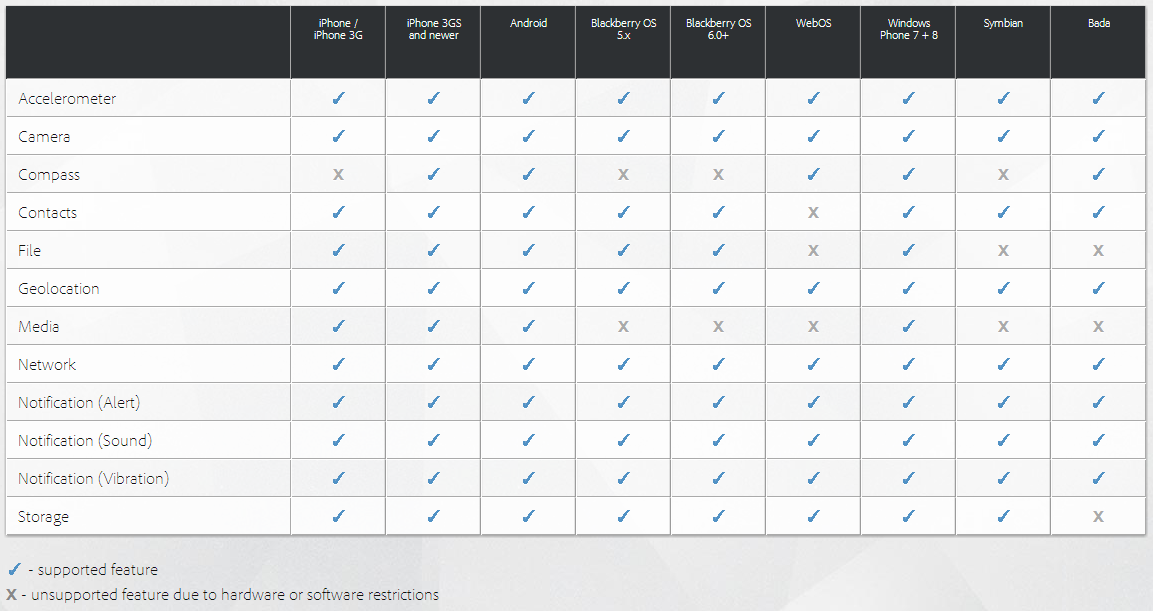
\includegraphics[width=1\textwidth]{Funzionalita}
	\caption{PhoneGap v2.7.0 - funzionalità supportate}						
	\label{fig:funzionalita}
\end{figure}

\subsection{Sistema di build delle applicazioni}

	Come già detto PhoneGap può essere visto come un framework atto a trasformare delle web application in applicazioni mobile fruibili su più piattaforme. Il build dell'app può avvenire in due modi:
	
\begin{itemize}
	\item \textbf{utilizzo di piattaforme specifiche}: la creazione di un applicazione con PhoneGap richiederà strumenti di sviluppo particolari a seconda della piattaforma su cui vogliamo rendere disponibile l'app. Per esempio se si volesse distribuire l'app su piattaforme iPhone, sarebbe necessario disporre di un computer apple con installato Xcode. Il sistema che andremmo a descrivere, si basa sull'uso di una piattaforma windows con lo scopo di distribuire l'app su sistemi android;
	
	\item \textbf{utilizzo di un build online}: Adobe ha creato un sistema di build online che permette di caricare il proprio codice sorgente o mediante un upload diretto, oppure specificando l'indirizzo di un repository Git contenente l'applicazione mobile. Questa scelta sicuramente comoda e da preferirsi alla prima, presenta però lo svantaggio di essere a pagamento, e di fornire gratuitamente il build di un unica applicazione. Per ulteriori informazioni rimandiamo al sito online: \url{https://build.phonegap.com/}.
\end{itemize}

\clearpage

\section{Configurare l'ambiente di lavoro}

I seguenti step per la configurazione dell'ambiente di lavoro prevedono l'utilizzo di un computer con sistema operativo Windows 7.

Lo sviluppo delle applicazioni si baserà sull'uso del framework JavaScript Sencha Touch 2, idealmente pensato per lo sviluppo mobile.

La soluzione proposta è ottenuta con strumenti gratuiti. Solo al termine di tale sezione saranno proposte alternative a pagamento.

\subsection{Strumenti necessari}

Prima di procedere con l'installazione e la configurazione dell'ambiente di lavoro, si raccomanda di effettuare il download del seguente materiale:

\begin{itemize}
	\item \textbf{JDK}: per sviluppare le nostre mobile application necessitiamo del Java Delelopment Kit, scaricabile all'indirizzo \url{http://www.oracle.com/technetwork/java/javase/downloads/jdk7-downloads-1880260.html}. Si osservi che la JDK contiene già la JRE, che di conseguenza non dovrà essere scaricata. Alla data corrente, l'ultima versione disponibile (che corrisponde anche a quella usata) è la 7. Nel sito troverete il link al download nella lista \textbf{Java SE Development Kit 7u21}. Nel nostro caso è stata usata quella per  Windows x64;
	\item \textbf{IDE Eclipse}: il software è reperibile al sito \url{http://www.eclipse.org/downloads/}. Per quanto la scelta tra le diverse versioni non dovrebbe comportare alcun problema, si raccomanda il download di \textbf{Eclipse IDE for Java EE Developers}. Alla data corrente, l'ultima versione (che corrisponde anche a quella utilizzata in questa guida) è Juno (4.2);
	\item \textbf{PhoneGap SDK}: potrete scaricare l'ultima versione  direttamente dal sito ufficiale di PhoneGap: \url{http://phonegap.com/download/};
	\item \textbf{ANT}: potrete scaricare il software direttamente dall'indirizzo \url{http://ant.apache.org/bindownload.cgi};
	\item \textbf{Android SDK}: potrete scaricare il software direttamente dal sito \url{http://developer.android.com/sdk/index.html};
\end{itemize}

Ora se siete intenzionati a sviluppare le vostre applicazioni con Sencha Touch 2, come proposto in questo manuale, necessitate di scaricare anche la sua SDK. Potrete reperirla direttamente dal sito ufficiale: \url{http://www.sencha.com/products/touch/download/}. Qui, fornendo il vostro indirizzo e-mail, potrete scaricare la versione gratuita. Se si desidera un ambiente di sviluppo completo, si può scaricare la versione a pagamento che fornisce:
\begin{itemize}
	\item Sencha Architect;
	\item Sencha Ext JS;
	\item Sencha Touch (si tratta del SDK che potete scaricare gratuitamente al link citato in precedenza);
	\item Sencha Eclipse Plugin;
	\item Sencha Touch Charts;
	\item Sencha Mobile Packaging;
	\item Enterprise Data Connectors;
	\item Sencha Support Package;
\end{itemize}

Bene, ora siamo pronti per iniziare!

\subsection{Installazione step by step}

\textbf{ATTENZIONE}: come vedrete in seguito, sarà necessario creare delle variabili di sistema. Ciò richiederà da parte vostra di inserire il percorso a determinati file. Dunque è importante tenere traccia dei percorsi d'installazione dei vari componenti.

\begin{description}
	\item[Step 1 - installare la JDK]: portiamoci nella cartella in cui abbiamo scaricato la JDK e avviamo l'installazione. Come già detto premuriamoci di prendere nota del path di installazione.
	\item[Step 2 - installare IIS]: andate dal menù Start e aprite il pannello di controllo. Quindi selezionate la voce programmi e dal menù che comparirà selezionate la voce Funzionalità di windows. Dopo un breve caricamento comparirà un elenco di funzionalità aggiuntive del sistema. Cercare la voce Internet Informarion Services, espandete l'elenco e selezionate Servizi Web e Strumenti di gestione Web. Terminate quindi l'installazione premendo su OK. Poi procedete aprendo ISS manager (ricercabile dalla strumento di ricerca presente nello start). Qui dovrete aggiornare il catalogo MIME aggiungendo l'estensione 'JSON' per le applicazioni 'application/json'. Se avete dubbi su tale procedura, potete consultare la discussione \url{http://stackoverflow.com/questions/332988/get-iis6-to-serve-json-files-inc-post-get/1121114#1121114 }.
	\item[Step 3 - installare Eclipse]: come per la JDK, portiamoci nella cartella in cui abbiamo scaricato Eclipse e scompattiamo l'applicativo nella cartella Programmi di windows. L'applicativo non richiede installazioni ed è già pronto per l'esecuzione.
	\item[Step 4 - installare Android-SDK]: avviate l'installazione della SDK scaricata in precedenza. Quindi aprite la SDK manager e cercate nell'elenco l'ultima versione di Android. Questa dovrebbe risultare già installata. Se cosi non fosse, spuntate la check box adiacente a tale voce e procedete con l'installazione. Quindi, sempre da SDK manager, spuntate la voce Tools e avviate l'installazione.
	\item[Step 5 - installare il plugin Android ADT]: aprite Eclipse e dal menù a tendina seguite il percorso Help > Install New Software... quindi nella text box nominate 'Work With' scrivete https://dl-ssl.google.com/android/eclipse. Quando vedrete comparire l'opzione install Developer Tools, cliccate su di essa e avviate l'installazione di tutti i componenti correlati a tale voce.
	\item[Step 6 - configurare le variabili d'ambiente] : come accennato all'inizio di questa sezione, è venuto il momento di impostare le variabili di sistema necessarie. Quindi facciamo click destro sull'icona 'Computer' (se non è presente un collegamento sul vostro Desktop, potrete trovarla nell'esplora risorse sulla colonna di sinistra). Procediamo selezionando la voce 'Proprietà'. Quindi andiamo su 'Impostazioni di sistema avanzate'. Si aprirà una finestra contenente un group panel. Andate alla voce avanzate e cercate il bottone nominato 'Variabili d'ambiente'. Cliccatelo e aggiungete nelle variabili di sistema la variabile JAVA\_HOME. Se per un qualche motivo non avete preso nota della cartella d'installazione di java, potete provare a cercare in \verb|C:\Program Files\Java\jdk1.7.0_21|.
	
	Ora cercate la variabile di sistema denominata path e aggiungetevi i seguenti percorsi (ogni percorso va separato da un ; ) relativi ai file:
	\begin{itemize}
		\item javac;
		\item ant;
		\item adb (NOTA: il percorso è relativo ad adb.exe, e lo troverete nella cartella platform-tools presente nella directory d'installazione della andrid sdk);
		\item android (NOTA: troverete il file nella cartella d'installazione della SDK di Andorid).
	\end{itemize}
	
	Se avete trovato difficoltà in tale sezione potete leggere il toutorial \url{http://simonmacdonald.blogspot.ca/2012/11/getting-create-command-to-work-on.html} che riporta delle soluzioni a tali problematiche.

\end{description}

Congratulazioni, a questo punto l'ambiente di lavoro è correttamente configurato!

\clearpage

\section{Sencha Touch 2}
\subsection{Introduzione al framework}

\begin{figure}[h]
	\centering
	
\includegraphics[width=0.2\textwidth]{sencha}
	\caption{Sencha Touch - logo}						
	\label{fig:sencha logo}
\end{figure}

Sencha Touch è un framework JavaScript avente architettura MVC, e il suo utilizzo è particolarmente adatto alla realizzazione di mobile application ibride. Tra le sue caratteristiche c'è la capacità di sviluppare applicazioni con il look and fell nativo delle principali piattaforme mobile. Tutto ciò avviene semplicemente caricando un apposito css nella pagina index.html dell'applicativo. 

Sencha basa il proprio funzionamento sull'Ext.JS e dispone di alcune componenti grafiche appositamente ottimizzate per un input di tipo touch. 

Volendo fornire una visione generale dell'architettura di Sencha, evidenziamo le seguenti componenti:

\begin{itemize}
	\item \textbf{Ext.Container - [View]}: sono le viste della nostra applicazione e sono definibili come dei contenitori di componenti grafici;
	\item \textbf{Ext.data.Model - [Model]}: rappresentano il modello dei dati. Quando definiamo un model definiamo i campi che lo caratterizzano e la loro natura (tipologia, parametri di default, opzionalià di inserimento, ecc...). Idealmente possiamo pensare ad un model come allo schema di una tabella di un database. Quando definiamo un Model dobbiamo definire anche la \textbf{tipologia della sorgente} fisica da cui estraiamo e su cui memorizziamo i dati. 
	\item \textbf{Ext.data.proxy.Proxy - [Proxy]}: rappresenta la tipologia di sorgente fisica espressa al punto precedente. Un proxy in associazione ad un Model, definisce come i dati vengono gestiti fisicamente dal browser e (nel caso siano usati su una applicazione ibrida) dal dispositivo portatile. Per esempio un proxy può essere di tipo JsonP, stabilendo quindi che la sorgente dei dati è fisicamente presente in un server esterno al dominio in cui risiede l'applicativo.
	\item \textbf{Ext.data.Srore - [Store]}: rappresenta un "contenitore" per la memorizzazione di dati. i dati memorizzati devono essere conformi allo schema espresso da un model, dichiarato in fase di definizione dello Store. Uno Store è un oggetto che può essere facilmente associato ad un componente della vista (come per esempio una lista). Sencha predispone una relazione Store-Vista simile a quella definita dal pattern observer, e garantisce quindi una sincronizzazione automatica della vista al variare dei dati presenti nello store.
	\item \textbf{Ext.app.Controller - [Controller]}: è l'oggetto contenente la logica di gestione dei dati. In una buona programmazione, il controller dovrebbe essere colui che fa interagire la vista con i dati sottostanti (pensando ad un'architettura MVC) e che sa far corrsispondere ad ogni evento il giusto gestore.
\end{itemize}

\subsection{L'architettura delle classi}
Prima di iniziare con la trattazione del argomento, informo il lettore che quanto mi accingo a trattare costituisce un breve riassunto del elaborato ``The Sencha Class System'', aggiornato con quanto da me sperimentato durante lo stage. 

Detto ciò voglio ricordare che Sencha Touch non è un linguaggio di programmazione object oriented. Pertanto egli non ha un concetto di programmazione a classi ben definito come in altri linguaggi (vedi per esempio Java). Sencha cerca tuttavia di predisporre degli oggetti il cui funzionamento e scopo emulano quasi alla perfezione quello delle classi, dando un esperienza d'uso che facilita lo sviluppatore nel compito di imporre una buona organizzazione strutturale al codice dell'applicativo. Nello specifico Sencha predispone un oggetto base denominato Ext.Class a cui possiamo riferirci quando, l'oggetto che stiamo definendo non deve ereditare nessun oggetto particolare già esistente. Per creare tali entità è possibile usare una sintassi simile alla seguente:

\lstset{language=java,caption={Esempio creazione di una Ext.Class in Sencha},label=DescriptiveLabel}
\begin{lstlisting}
var Person = new Ext.Class({
    name: 'Mr. Unknown',
    walk: function(steps) {
        alert(this.name + ' is walking ' + steps + ' steps');
    }
});
\end{lstlisting}

Come si può osservare l'oggetto Ext.Class accetta come unico parametro un oggetto costituito da coppie chiave-valore. In tale contesto le chiavi devono essere univoche e i valori associati possono essere sia oggetti, tipi primitivi o funzioni. In un certo senso cosi facendo è possibile definire ``inline'' la struttura di un oggetto specificandone le variabili e i metodi pubblici. Mediante la \emph{keyword}.

Come ogni classe degna di questo nome, anche in Sencha è possibile definire un costruttore per l'inizializzazione delle istanze della classe. Per farlo si usa la \emph{keyword} come nel seguente modo:

\lstset{language=java,caption={Definire un costruttore per le classi Sencha},label=DescriptiveLabel}
\begin{lstlisting}
var Person = new Ext.Class({
    name: 'Mr. Unknown',
 
    //costruttore pubblico della classe
    constructor: function(name) {
        this.name = name;
 
        return this;
    },
 
    walk: function(steps) {
        alert(this.name + ' is walking ' + steps + ' steps');
    }
});

//creo un'istanza di persona usando il costruttore 
var jacky = new Person('Jacky');
jacky.walk(10); // alerts "Jacky is walking 10 steps"
\end{lstlisting}

\subsubsection{Ext.define()}
Ovviamente un sistema di definizione delle classi come quello proposto in precedenza è sconsigliabile, e da usare solo quando Sencha non ci permette di usare l'oggetto Ext.define(). Questo infatti ci permette di definire lo schema di un oggetto (ci permette di emulare una classe) in un file separato dal resto del codice in cui l'oggetto viene istanziato. Ext.define() accetta 3 parametri:

\begin{itemize}
	\item una stringa rappresentante il nome della classe;
	\item un oggetto analogo a quello usato in Ext.Class, contente le coppie chiave-valore usate per definire la struttura dell'oggetto;
	\item una funzione di callback da invocare quando tutte le dipendenze della classe sono state risolte;
\end{itemize}

Un esempio di utilizzo di tale sistema è il seguente:

\lstset{language=java,caption={Usare Ext.define()},label=DescriptiveLabel}
\begin{lstlisting}
Ext.define('My.sample.Person', {
    name: 'Mr. Unknown',
 
    constructor: function(name) { /* ... */ },
 
    walk: function(steps) { /* ... */ }
});
\end{lstlisting}

Per istanziare un oggetto a partire da unaclasse cosi definita, è sufficiente utilizzare la già citata funzione Ext.Class(), passando:
\begin{itemize}
	\item come primo parametro il nome completo della classe o l'alias con cui è stata definita;
	\item come secondo parametro (se la classe lo richiede) l'oggetto di configurazione usato dal costruttore ridefinito.
\end{itemize}

\subsubsection{Namespacing}
Come nella progettazione di ogni applicativo, usare un approccio orientato agli oggetti ci permette di definire le classi cui si compone l'applicativo stesso. Mediante il sistema di emulazione delle classi fornito da Ext.define() ciò è possibile anche con Sencha. Di conseguenza possiamo strutturare le componenti dell'applicazione mediante una suddivisione in package e l'ovvio ordinamento dei nomi mediante namespacing. Ciò si ripercuote sulla nomenclatura che usiamo sulla classe. Tale infatti deve rispettare la posizione che essa ha nel package in cui è collocata. Per esempio se abbiamo il package MyCompany/MyTool/yClass, la classe MyClass dovrà essere nominata nel Ext.define() come: MyCompany.MyTool.MyClass.

\subsubsection{Pre \& post-processors}
Prima di creare ed eseguire una classe da noi definita, vi è un'attività della pre-processors in cui il codice della classe viene esaminato alla ricerca di determinate parole chiave. Tra queste \emph{keyword} cito:
\begin{itemize}
	\item \textbf{extend}: property usata per emulare il meccanismo di ereditarietà tra classi;
	\item \textbf{mixins}: property usata per far si che la classe definita contenga anche il contenuto delle classi specificate in tale proprietà;
	\item \textbf{config}: property in cui vengono definite coppie chiave-valore per le quali il meccanismo di pre-processors definisce metodi di set e di get in automatico;
	\item \textbf{requires}: property usata per definire una serie di elementi esterni richiesti dalla classe per i suoi scopi (simile al meccanismo di import delle classi in Java);
	\item \textbf{statics}: property che permette di definire delle variabili e delle funzioni statiche;
\end{itemize}
Analogamente ai pre-processors esistono dei post-processors, ossia delle parole chiave (con funzioni ben precise) che vengono processate a run-time solo quando la classe è pronta. Tra queste menziono:
\begin{itemize}
	\item \textbf{singleton}: emulazione del pattern singleton, usata quindi per limitare il numero di istanze creabili ad una;
	\item \textbf{alternateClassName}: permette di definire un nome alternativo con cui riferirsi alla classe. Generalmente usata per garantire una retro-compatibilità per le classi rinominate;
    \item \textbf{alias}: genera un xtypes che viene mappato nel contesto dell'applicazione. Tale alias può essere usato in un qualsiasi punto come \emph{shorthands} (abbreviazione) per riferirsi alla classe stessa.
\end{itemize}

\subsection{Best practice}

\subsubsection{Creare un progetto}

Per creare una buona applicazione e lavorarvi nell'ordine, è importante impostare correttamente l'ambiente di lavoro. Innanzitutto portiamoci nella directory root del web browser su cui lavoriamo. Nel nostro caso la cartella si trova in \verb|C:\intpub\wwwroot|. Qui creiamo una cartella con il nome del nostro progetto (con riferimento all'app che creeremo nella sezione "La mia prima applicazione") NotesApp. Quindi definiamo al suo interno:

\begin{itemize}
	\item una cartella app che conterrà la struttura vera e propria dell'applicativo. LA cartella conterrà a sua volta:
	\begin{itemize}
		\item una cartella view;
		\item una cartella controller;
		\item una cartella store;
		\item una cartella model;
		\item (opzionale... diventa obbligatorio se si vuole ridefinire un Ext.data.proxy.*) una cartella proxy.\\
		
		Le cartelle cosi create andranno a contenere i file che definiscono gli omonimi oggetti Sencha precedentemente descritti;
	\end{itemize}
	\item una cartella lib che conterrà la libreria Sencha Touch 2;
	\item una cartella rsc (o resorces se preferite), dove caricheremo i css personali;
	\item un file index.html;
	\item un file app.js;
	\item (per ora facoltativo... diventa obbligatorio se vogliamo trasformare la web app in un app ibrida fruibile su device portatili) copiare il file cordova cordova-2.7.0.js, scaricabile insieme all'ultima versione di PhoneGap.
\end{itemize}

Detto ciò, per dare una trattazione maggiore sull'utilizzo dei vari file creati, rimandiamo alla guida riportata in sezione "La mia prima applicazione".

\subsubsection{In linea generale}

La logica di sviluppo di un applicazione Sencha, non che il sistema con cui si "incastrano" le varie componenti fin qui presentate, dovrebbe essere quella di:
\begin{itemize}
	\item progettare e predisporre la grafica dell'applicazione tramite la definizione di un layout e dei componenti costituenti le view.
	\item definire i modelli dei dati su cui lavorare, stando attenti a scegliere la tipologia giusta di proxy (lo sviluppatore non si spaventi, passare da un tipo di proxy ad un'altro in corso d'opera, è un azione semplice quanto sostituire una stringa);
	\item definire gli store necessari scegliendo con cura se gestirli con un auto load o nel caso assicurandosi di caricarli nel momento giusto;
	\item associare gli store alle componenti delle view predisposte per la visualizzazione dei dati;
	\item definire degli eventi da associare ai componenti della vista;
	\item predisporre un uno o più controller. Idealmente, sia per chiarezza che per manutenibilità, si definisce un controller per ogni view dell'applicazione;
\end{itemize}

\subsubsection{Come definire e sfruttare il meccanismo delle classi}
L'argomento è in se molto corposo, ed una trattazione cosi esaustiva esula dagli scopi di questo documento. Si raccomanda di leggere l'articolo riportato all'indirizzo \url{http://www.sencha.com/learn/sencha-class-system}.

Data l'importanza di alcuni accorgimenti, si riportano di seguito solo alcune delle funzionalità riportate nell'articolo precedentemente citato:
\begin{description}
	\item[Config e la definizione automatica di getter e setter]: ogni classe di Sencha definisce al suo interno un oggetto config, strutturato come una raccolta di property. Il framework predispone per ogni property qui definita, un getter ed un setter facente riferimento al nome della property stessa. Quindi se si definisce config{ myName: 'Andrea' }, sarà possibile richiamare pubblicamente getMyName(). Si osservi come la prima lettera della property, nel getter, diventi maiuscola.
	\item[Richiamare un metodo di super dentro l'override dello stesso]: se vi trovate ad estendere una classe di Sencha, può essere necessario ridefinire un comportamento specifico per un metodo della superclasse, che al suo interno preveda un caso di default la cui gestione debba essere delegata allo stesso metodo della superclasse (quindi al metodo non sovrascritto). Un esempio potrebbe essere la ridefinizione del metodo load() di uno store. Supponendo di voler gestire in modo diverso il primo load, potremmo sovrascrivere il metodo andando a specificare un comportamento per il nostro caso, richiamando negli altri il load di super. Una procedura del genere si esegue inserendo, all'interno del metodo sovrascritto, l'istruzione \texttt{this.callParent()}. Si osservi infine che se il metodo richiamato necessità di parametri la dicitura diventa \texttt{this.callParent(arguments)}.
\end{description}

\subsubsection{Come usare le associazioni tra modelli}
Sencha permette di definire 3 diverse tipologie di associazione tra modelli:
\begin{itemize}
	\item \textbf{hasOne}: serve per indicare che un istanza del modello è associata ad una ed una solo istanza del modello a cui è associata (e.g. una macchina ha uno ed un solo motore -> car hasOne engine);
	\item \textbf{hasMany}: serve per indicare un associazione multipla. L'istanza di partenza è associata a zero o più istanze del modello associato (e.g. una macchina ha più ruote -> car HasMany tyre);
	\item \textbf{belongsTo}: indica un rapporto di appartenenza unitario, del tipo padre-figlio (e.g una macchina appartiene ad uno ed un solo proprietario -> car belongsOne owner).
\end{itemize}

\begin{figure}[h]
	\centering
	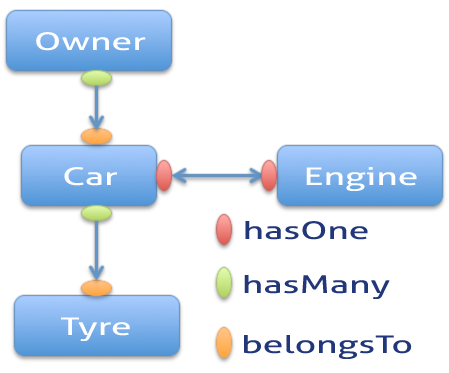
\includegraphics[width=0.5\textwidth]{associazioni}
	\caption{Sencha Touch - associazioni tra modelli}						
	\label{fig:associazioni}
\end{figure}

Quanto detto si traduce in codice nel seguente modo:
\lstset{language=java,caption={Esempio di associazioni tra modelli},label=DescriptiveLabel}
\begin{lstlisting}
Ext.define("MyApp.model.Car", {
    extend: 'Ext.data.Model',
    config: {
        idProperty: 'Id',
        fields: [
            { name: 'Id' },
            { name: 'brandName' },
            { name: 'type' },
            { name: 'ownerId' }
        ],
        belongsTo: [{ model: 'MyApp.model.Owner', associationKey: 'ownerId' }],
        hasOne: [{ model: 'MyApp.model.Engine', associationKey: 'engineId' }],
        hasMany: [{ model: 'MyApp.model.Tyre' }]
    }
});
\end{lstlisting}

Tutto ciò risulta di grande interesse perché ci permette di avvicinare sempre di più il nostro codice a quella che è la forma del modello logico del DB. Tuttavia dagli studi eseguiti emerge una mancanza significativa negli automatismi offerti da Sencha. Supponendo di creare uno store che si basa sulla memorizzazione di istanze di tyre, vogliamo definire una vista a cui associarlo, e in cui visualizzare direttamente non solo i dati dei pneumatici, ma anche i dati contenuti nei modelli associati, che per l'appunto, si basano su di un proxy di tipo JsonP (per ulteriori informazioni vedi "Approfondimento sui proxy"). Per esempio vogliamo che ogni item della lista visualizzi il nome del pneumatico, l'id della macchina associata e il nome del proprietario della macchina. Tutto ciò risulta essere problematico.

\begin{description}
	\item[Il problema]: analizzando in dettaglio il problema osserviamo quanto segue. Quando viene eseguito il comando load dello store, questi carica i dati dal server remoto usando le informazioni di configurazione del proxy. In molti casi però il caricamento dei dati è asincrono. Questo significa che i record dei pneumatici e delle auto saranno istanziati senza conoscere le loro controparti correlate. Così, quando abbiamo recuperare un record Tyre dallo store, questi non ha alcun riferimento al record (padre) auto, che vorremo utilizzare nel componente List. L'unico modo per farlo è quello di caricare l'intera struttura dati dei proprietari (owner), compresi i "figli" di car e di tyre, in un singolo passaggio e utilizzando una struttura dati "ibrida". In pratica questo metodo di caricamento dei dati è ingombrante e per lo più non supportato dalle tipiche backend's API.
	\item[La soluzione]: una soluzione al problema è stata trovata da due sviluppatori: Rob Boerman e Aaron Smith. Questi l'hanno pubblicata nel proprio sito web, raggiungibile all'indirizzo riportato al termine di questo paragrafo. Essa consiste nel ridefinire un modello "base" che provvede all'inizializzazione delle associazioni (agli altri modelli), quando una componente (per esempio una lista) necessita dei dati. Ciò si traduce nell'istruire il modello su come rintracciare i dati associati.
	Osservando che uno dei metodi principali per ottenere dati a partire da uno store è il metodo getData(), gli sviluppatori sopramenzionati hanno optato per un ovverride del metodo stesso, che prevedesse per l'appunto le informazioni su come ottenere i dati associati. Quindi ogni modello del sistema sarà creato come estensione di questo modello base.
\end{description}

Poiché una trattazione estesa di questo argomento, esula dagli scopi del documento, si rimanda al seguente link per ogni approfondimento:
\url{http://appointsolutions.com/2012/07/using-model-associations-in-sencha-touch-2-and-ext-js-4/}

Come si potrà osservare, quanto qui riportato è un piccolo estrapolato dell'articolo.

Prendendo in considerazione altre soluzioni, più facile da pensare ma decisamente più onerosa in termini di tempo di elaborazione, si osserva la possibilità di definire ad hoc delle richieste Ajax al server per ottenere tutti i dati necessari.

\subsubsection{FireEvent: una gestione intelligente degli eventi}
In un ottica di programmazione basata su pattern architetturale MVC, la vista è svincolata dal conoscere le regole di business attuate per modificare i dati in relazione al verificarsi di un determinato evento. Infatti dovrebbe essere compito del controller mettersi in "ascolto", su delle view di cui è responsabile, ed essere pronto a catturare gli eventi sollevati dai componenti delle view. Quindi il controller potrà associare agli eventi il giusto \textit{handler}, per la risoluzione del medesimo.

Sencha permette di gestire tale procedura nel seguente modo:
\begin{itemize}
	\item[1)] si definisce un controller (in generale diciamo uno per ogni view), e si dichiarano le viste su cui dovrà mettersi in ascolto.
	\item[2)] quindi per ogni evento particolare, legato all'interazione dell'utente con un componente della view, si definisce una "delega" in un listener della vista (ciò avviene nella view stessa) il cui compito sarà delegare l'evento ad un \textit{handler} appropriato. la funzione \textit{handler} avrà poi il compito di sollevare un nuovo evento (convenzionalmente nominabile come ''comamand'') mediante l'evento FireEvent. Si osservi che in questa ottica la view non conosce direttamente chi la osserva, il che rende il codice molto più mantenibile. Analoga conclusione vale per il fatto che cosi facendo vi è una completa divisione tra logica e grafica.
	\item[3)] a questo punto di può tornare sul controller e dichiarare che la view x, su cui il controller è in ascolto, può sollevare l'evento y e che tale situazione si risolve delegando la gestione dell'evento ad una funzione appositamente creata. In linea generale se l'operazione riguarda la manipolazione di alcuni dati sensibili, ciò dovrebbe avvenire richiamando i metodi definiti nel model.
\end{itemize}

Per completezza riportiamo di seguito un esempio:\\

quella che segue è la vista, si osservi che 
\begin{itemize}
	\item[A)] è presente un listener che definisce le associazioni evento-componente-handler; 
	\item[B)] è presente un \textit{handler} associato all'evento tap del bottone;
	\item[C)] l'\textit{handler} non fa altro che sollevare un nuovo evento tramite metodo FireEvent.
\end{itemize}

\lstset{language=java,caption={Gestione degli eventi - sollevare un evento con FireEvent},label=DescriptiveLabel}
\begin{lstlisting}
//Vista NotesList -> rappresenta una lista di note. contiene un bottone NewNote il cui scopo consiste nell'effettuare una transizione verso la vista NoteEditor

Ext.define('NotesApp.view.NotesList',
{
	extend: 'Ext.Container',
	requires: ['Ext.dataview.List'],
	alias: 'widget.notesListView',
	
	config:
	{
		...
		items:
		[
			{
				xtype: 'toolbar',
				docked: 'bottom',
				items:
				[
					{ xtype: 'spacer' },
					{ 
						xtype: 'button',
						itemId: 'newButton',
						text: 'New Note',
						ui: 'action'
					},
					{ xtype: 'spacer' }
				]
			},	
			...
		]
		...
		
		//Listeners: usato per mettere la vista in ascolto di se stessa. L'idea consiste nel catturare gli eventi del tipo "iterazione dell'utente con le componenti della view"
		listeners:
		[
			{
				//componente da "ascoltare" identificato mediante id
				delegate: '#newButton',
				//tipologia di evento da "catturare"
				event: 'tap',
				//funzione "handler" per la risoluzione dell'evento
				fn: 'onNewButtonTap'
			},
			...
		]
	},
	
	//---------------FireEvent-------------------
	
	//Handler di #newButton - evento: tap
	onNewButtonTap: function()
	{
		console.log('newNoteCommand');
		//Sollevo l'evento newNoteCommand
		this.fireEvent('newNoteCommand', this);
	},
	
	...
});
\end{lstlisting}

Per completare l'esempio, riportiamo il codice commentato del controller. Qui vogliamo mettere in evidenza i seguenti punti:

\begin{itemize}
	\item[A)] il controller definisce una lista refs delle viste su cui restare in ascolto;
	\item[B)] il controller definisce, in una zona detta control, le coppie nome evento - command da richiamare;
	\item[C)] al termine del listato compaiono i command da richiamare per processare la richiesa inoltrata in princio dall'iterazione utente - componente della vista;
\end{itemize}

\lstset{language=java,caption={Gestione degli eventi - sollevare un evento con FireEvent},label=DescriptiveLabel}
\begin{lstlisting}
//Controller Notes -> controller della vista 

Ext.define('NotesApp.controller.Notes',
{
	extend: 'Ext.app.Controller',
	config:
	{
		//refs usato per tracciare i riferimenti nomeVista-aliasUsatoNelController
		refs:
		{
			//stabilisco che questo controller osserva gli eventi lanciati dall'oggetto xtype = noteListView
			notesListView: 'notesListView',
			...
		},
		
		//parte di controller. Per ogni vista gestita dal controller, definisce le coppie nomeEventoDaCatturare-nomeHandlerDelController
		control:
		{
			notesListView:
			{
				//definisco la lista degli eventi che possono essere lanciati (mediante fireEvent) dall'oggetto che sto osservanto (xtype: notesListView)
				newNoteCommand: 'onNewNoteCommand',
				...
				/*this ref automatically creates a getNoteEditor() function in the controller, which we can use to refer to the NoteEditor instance and make it the active View in the application.*/
			},
			...	
		}
	},

	//---------LISTA DEI COMANDI---------------
	
	//comando associato all'evento newNoteCommand dell'oggetto notesListView.
	onNewNoteCommand: function()
	{
		//istruzioni per risolvere l'evento. Nel caso, si tratta di istruzioni per creare una nuova nota vuota, ed effettuare uno shift di navigazione, alla view contenente l'editor di note.
	},
	...
});
\end{lstlisting}

\subsubsection{Gestire il multi-tap}

Come si può vedere dall'esecuzione di una qualsiasi app di Sencha, questo sono realizzate in modo tale da non provocare un blocco dell'interfaccia in seguito all'esecuzione di un comando dovuto alla pressione di un bottone. Cosi facendo l'utente ha la possibilità di navigare nell'interfaccia, mentre in background vengono svolte le operazioni da lui richieste. Ciò è possibile mediante un sistema di gestione degli eventi. Infatti quando premiamo, o se preferite, quando eseguiamo un tap su di un Ext.Button, viene generato un evento che sarà catturato da un handler da noi specificato. Questo sistema rende quindi asincrona ogni richiesta da noi fatta al sistema per mezzo di una componente grafica.

A questo punto molti sviluppatori non si avvedono di un potenziale problema di stabilità dell'applicativo. Se supponiamo l'utente di turno, per un qualche motivo, inizia a premere ripetutamente il pulsante A, questo provocherà una serie di fireEvent relativi all'evento tap che, catturati dall'handler, provocheranno l'esecuzione del blocco di codice designato. A ciò si aggiunge un ulteriore problema: JavaScript non gestisce la mutua esclusione. Non esistono quindi istruzioni atomiche da usare come ''barriera di sincronizzazione''.

Considerando quanto detto, si pensi allo scenario: un bottone A ha come handler associato una funzione di download che:

\begin{itemize}
	\item[1)] scarica i dati dal server;
	\item[2)] cancella quelli locali;
	\item[3)] salva i dati temporanei nello spazio di memoria locale.
\end{itemize}

In un tale contesto, se l'utente preme ripetutamente A, genererà diverse richieste di download. Un possibile risultato è che due processi eseguono in successione il passo 1) e il passo 2). A tal punto entrambi avrebbero cancellato due volte l'area di memoria locale, e si appresterebbero a sovrascriverci i dati dalla loro zona di memoria. Ciò provoca di conseguenza una ridondanza nei dati scaricati.

Purtroppo l'incapacità di JavaScript di eseguire blocchi di codice in mutua esclusione (si badi bene, semplici barriere di tipo if con variabili booleane non sono sufficiente) rende il nostro codice debole e potenzialmente pericoloso. Per fortuna, in seguito ad una domanda sul forum di Sencha, uno sviluppatore ha definito un Ext.Button in grado di accettare un unico tap in una serie di tap concatenati. Di seguito riportiamo il codice di tale componente.

\lstset{language=java,caption={org.s2.singleEventItem.button.SingleTapButton},label=DescriptiveLabel}
\begin{lstlisting}

Ext.define('org.s2.singleEventItem.button.SingleTapButton', 
{
    extend : 'Ext.Button',
    xtype  : 'stbutton',

    initialize : function() {
        var me = this;

        me.element.on({
            scope     : me,
            singletap : 'onSingleTap',
            doubletap : 'onDoubleTap'
        });

        me.callParent();
    },

    onSingleTap : function () {
        this.fireEvent('singletap', this);
    },

    onDoubleTap : function () {
        this.fireEvent('doubletap', this);
    }
});

\end{lstlisting}

Ora invece vediamo come usare tale componente. Per prima cosa creiamo nella nostra vista un bottone avente come xtype, quello del nostro SingleTapButton. Una tale operazione si fa, per esempio, nel seguente modo:

\lstset{language=java,caption={Usare il SingleTapButton - definire il bottone},label=DescriptiveLabel}
\begin{lstlisting}

...

{
	xtype: 'stbutton', //ora il nostro bottone accettera' il single tap.
	itemId: 'downloadButton',
	iconCls: 'download',
	iconMask: true,
	ui: 'action',
	scope: this
},

...

\end{lstlisting}

Passiamo quindi a definire l'handler da associare. Con il sistema appreso nella sezione del fireEvent, definiamo nella config della vista, un listener abilitato alla delega dell'evento singletap del nostro bottone:

\lstset{language=java,caption={Usare il SingleTapButton - listeners},label=DescriptiveLabel}
\begin{lstlisting}

listeners:
[
	...
			
	{
		delegate: '#downloadButton',
		event: 'singletap',
		fn: 'onDownload'
	},
	
	...
]
\end{lstlisting}

A questo punto basta definire la funzione onDownload, dalla quale genereremo un evento che sarà catturato da un apposito controller. Nel controller si definirà la parte di logica per la gestione dell'evento.

Per prendere nota del dibattito presente sull'argomento nel forum di Sencha, si rimanda al link:\\

\url{http://www.sencha.com/forum/showthread.php?208657-Multiple-taps-issue-BUG}

\subsubsection{Migliorare le performance di Sencha}

Sencha si è rivelato un framework dalle grandi potenzialità. Purtroppo però, il suo utilizzo mediante PhoneGap genera app piuttosto pesanti e non ben ottimizzate. Dopo diverse prove infatti si è osservato che su smatphone di fascia media (ovviamente rispetto al periodo in cui è scritto il documento ), le applicazioni costruite con tali framework risultavano essere piuttosto lente. Invece l'esecuzione su tablet ha dato esiti soddisfacenti. Comunque per cercare di migliorare il più possibile le app e i sorgenti che le compongono si consiglia di adottare le best practice riportate all'indirizzo sottostante:\\

\url{http://dionbeetson.blogspot.it/2012/10/sencha-touch-performance-tips-and-tricks.html}

\subsection{Eseguire test di unità su componenti Sencha}

\subsubsection{Syntax check}

Oggi giorno per garantire un prodotto software di qualità è necessario testarlo in più modi, affinché si possa stabilire con certezza che il suo comportamento è corretto. Tra le varie tipologie di test, la prima che merita di essere citata, è sicuramente la syntax check. Questa tecnica, che ritroviamo eseguita automaticamente nei linguaggi compilati, al momento della compilazione, ci permette di rilevare errori sintattici nel codice. JavaScript non essendo un linguaggio che richiede compilazione, non offre la possibilità di individuare gli errori, se non eseguendo il codice stesso. Inoltre si osservi che a molti piccoli errori, è il browser stesso a porvi rimedio. Questo infatti è il caso dei '';'' presenti al termine delle istruzioni JavaScript. 

Quindi per offrire allo sviluppatore uno strumento valido al fine di rilevare ogni genere di errore, uno sviluppatore della Sencha.inc ha ideato un programma eseguibile da shell, che data una directory principale e una lista di sotto-directory da escludere durante l'attività di check, si occupa di esaminare ogni file con estensione .js usando il tool JsLint (\url{http://www.jslint.com/}). Per un'approfondimento sul tema, comprese le istruzioni per mettere in pratica tale tecnica, rimandiamo al link \url{http://www.sencha.com/blog/automating-unit-tests}.

\subsubsection{Configurare Jasmine per testare Sencha}

Come prima cosa è importante configurare correttamente l'ambiente di lavoro. Iniziamo scaricando la versione stand-alone di Jasmine, all'indirizzo \url{https://github.com/pivotal/jasmine/downloads}. Quindi scompattiamo il contenuto del pacchetto .zip nella cartella /test/unitTest della directory principale del nostro progetto. Procediamo quindi seguendo il seguente iter:
\begin{itemize}
	\item[1)] definiamo all'interno della cartella /test/unitTest una cartella spec, dove andremo a inserire i file .js che definiscono le test suit;
	\item[2)] creiamo un file app-test.js che andremo a mettere nella stessa directory in cui si trova l'app.js della nostra applicazione;
	\item[3)] infine andiamo a creare un file run-test.html.
\end{itemize}

A questo punto procediamo procediamo andando a scrivere il contenuto di app-test.js. Questo file rappresenta  il file centrale per il caricamento delle componenti da testare e per l'avvio del kernel di Jasmine. App-test.js può essere scritto nel seguente modo:

\lstset{language=java,caption={Template di app-test.js},label=DescriptiveLabel}
\begin{lstlisting}
Ext.application({
	//elenco di modelli e store necessari per il testing
	//Per esempio:
	models: ['Note','Author'],
	stores: ['Notes'],
	
	requires: 
	[
		//elenco delle classi richieste per l'esecuzione del test.
		//Per esempio:
		'org.s2.syncEngine.SyncManager',
		'org.s2.syncEngine.basicSyncStore.download.DownloadStoreFactory',
		'org.s2.syncEngine.basicSyncStore.upload.CommitStoreFactory',
		'org.s2.syncEngine.basicSyncStore.storeCommand.AddCommit',
		'org.s2.syncEngine.basicSyncStore.storeCommand.UpdateCommit',
		'org.s2.syncEngine.basicSyncStore.storeCommand.DeleteCommit',
		'org.s2.syncEngine.basicSyncStore.SyncStore',
		'NotesApp.model.Author',
	],
	
	//Per evitare la generazione del viewport
	autoCreateViewport: false,
	
	//nome dell'app
	name: 'NotesApp',
	
	//Lancher di app-test. Usare sempre questo template
	launch: function() 
	{
		jasmine.getEnv().addReporter(new jasmine.TrivialReporter());
		jasmine.getEnv().execute();
	}
});
\end{lstlisting}

Quindi procediamo definendo il file run-test.html:

\lstset{language=java,caption={Esempio di run-test.html},label=DescriptiveLabel}
\begin{lstlisting}
<html>
	<head>
		<meta charset="UTF-8">
		<!-- i commenti indicano cosa inserire nelle varie parti. I dati non commentati sono lasciati per esempio-->
		<title>NotesApp unit test - Jasmine</title>
		<!-- Jasmine css file: carica il css di Jasmine-->
		<link rel="stylesheet" type="text/css" href="app-test/lib/jasmine-1.3.1/jasmine.css">
		<!-- <x-bootstrap> inseirisci qui la libreria sencha-->
		<script src="lib/ST2/sencha-touch-all-debug.js"></script>
		<!-- Jasmine js files -->
		<script type="text/javascript" src="app-test/lib/jasmine-1.3.1/jasmine.js"></script>
		<script type="text/javascript" src="app-test/lib/jasmine-1.3.1/jasmine-html.js"></script>
		<!-- App css files -->
		<link rel="stylesheet" href="./lib/ST2/resources/css/sencha-touch.css" type="text/css">
		<link rel="stylesheet" href="./resources/css/app.css" type="text/css">
		<!-- application source files -->
		<script src="app-test.js"></script>
		<!-- / application source files: inserisci qui gli spec per il testing delle singole componenti -->
		<script type="text/javascript" src="app-test/spec/IndexIDStoreSpec.js"></script>
		<script type="text/javascript" src="app-test/spec/IndexIDStoreFactorySpec.js"></script>
		<script type="text/javascript" src="app-test/spec/DownloadStoreFactorySpec.js"></script>
		<script type="text/javascript" src="app-test/spec/CommitStoreFactorySpec.js"></script>
		<script type="text/javascript" src="app-test/spec/AddCommitSpec.js"></script>
		<script type="text/javascript" src="app-test/spec/UpdateCommitSpec.js"></script>
		<script type="text/javascript" src="app-test/spec/DeleteCommitSpec.js"></script>
		<script type="text/javascript" src="app-test/spec/SyncStoreSpec.js"></script>
		<script type="text/javascript" src="app-test/spec/SyncManagerSpec.js"></script>
	</head>
	<body></body>
</html>
\end{lstlisting}

Ora l'ambiente è configurato. Non dobbiamo fare altro che costruire le nostre spec e metterle nell'omonima cartella definita al punto 1. Per eseguire i test basta richiamare dal browser all'indirizzo localhost il file run-test.js.

\subsubsection{Unit test - intoduzione}

La seconda tipologia di test, più interessante e atta a rilevare comportamenti anomali nelle componenti che costituiscono l'applicativo, prende il nome di \textbf{unit test}. Questa tecnica si basa sulla seguente considerazione: quando scriviamo del codice, lo facciamo sapendo già quali modifiche esso apporterà al sistema nei vari casi di esecuzione. Quindi il blocco di codice da testare avrà un suo \emph{valore atteso} che non necessariamente sarà uguale al suo \emph{valore effettivo}, ossia quello che rileviamo in fase di esecuzione. Tale anomalia è dovuta ad un nostro errore. I test di unità quindi, basandosi su un valore atteso (da noi specificato), eseguono il blocco di codice da testare e al termine verificano, con una certa tipologia di comparazione (uguale a, diverso da, maggiore di, ecc...) da noi specificata, se il valore ottenuto è conforme a quello atteso.

Creare ed eseguire test di unità per sorgenti JavaScript è un'operazione avviabile  con diversi tool. Per la sua semplicità, per la chiarezza di linguaggio e per le potenzialità offerte (e.g. facilitazioni nel test di blocchi asincroni) questa guida si rifarà al tool Jasmine. Poiché una trattazione approfondita sulle basi di Jasmine esula dallo scopo di questa sezione si rimanda il lettore all'appendice C, dove potrà trovare un mini-tutorial e dei link utili. Di seguito parleremo delle best practice da adottare nel testing si Sencha, dando per scontata la conoscenza di Jasmine.

\subsubsection{Best practice per il testing degli store}

Quando testiamo uno store è sempre molto utile definire una funzione per creare lo store, e tramite le apposite funzioni beforEach e afterEach, provvedere alla sua creazione (All'inizio di ogni singolo test) e alla sua eliminazione (alla fine del test). Per rendere meglio questo concetto proponiamo il seguente template:

\lstset{language=java,caption={Template per il testing degli store},label=DescriptiveLabel}
\begin{lstlisting}

describe("NomeStoreSpec", function() 
{
	//classe contenente che definisce lo store
	var storeCreator = function()
	{
		var myoStore = Ext.create('AliasStore');
		return myoStore;
	};
	
	//istanza di store usata per i test
	var store = null;
	
	beforeEach(function()
	{
		//ad ogni test creo lo store
		if (!store) 
		{
			store = storeCreator();
			store.load();
		}
		expect(store).toBeTruthy();
		waitsFor(function(){ return !store.isLoading(); },"load never completed", 4000);
	});
	
	afterEach(function()
	{
		store.getProxy().dropTable();
		store = null;
	});
	
	...
	
	//elenco di it() ... 
});
\end{lstlisting}

Per quanto riguarda invece i test da eseguire, si raccomanda di assicurarsi come prima che lo store sia stato caricato con successo. Quindi si procede verificando che il modello utilizzato dallo store corrisponda a quello che si è assegnato. Ciò potrebbe sembrare banale, ma è comunque un test da fare, specie per gli store più elaborati da noi ridefiniti. Analogamente è importante osservare che il proxy usato dallo store sia del tipo atteso. Proponiamo di seguito un esempio di come possono essere riportati due it del genere:

\lstset{language=java,caption={Template per il testing degli store - it di base},label=DescriptiveLabel}
\begin{lstlisting}

it('IndexIDStore caricato con successo', function()
{
	var isLoaded = store.isLoaded();
	expect(isLoaded).toBe(true);
});
 
it("Model dello store valido (type: NOME_MODELLO)",function()
{	
	var modelloStore = store.getModel().getName();
	var modelloAtteso = 'PATH_COMPLETA_DEL_MODELLO';
	//e.g PATH_COMPLETA_DEL_MODELLO = 'org.s2.MioStore.MioModello'
	
	expect(modelloStore).toBe(modelloAtteso);
});

it("Proxy type di store valido (type: TIPO_ATTESO)",function()
{	
	var proxyTypeStore = store.getProxy().config.type;
	var proxyTypeAtteso = 'TIPO_ATTESO';
	//e.g TIPO_ATTESO = 'sql'

	expect(proxyTypeStore).toBe(proxyTypeAtteso);
});

\end{lstlisting}

\subsubsection{Approfondimenti}

Per ulteriori approfondimenti sul tema, si rimanda ai seguneti link:
\begin{itemize}
	\item \textbf{Tutorial del Pivotal Lab}: guida completa che spiega come eseguire test di unità su codice Sencha. I link per le varie parti sono:\\
		\url{http://pivotallabs.com/sencha-touch-bdd-part-1/}\\
		\url{http://pivotallabs.com/sencha-touch-bdd-part-2/}\\
		\url{http://pivotallabs.com/sencha-touch-bdd-part-3/}\\
		\url{http://pivotallabs.com/sencha-touch-bdd-part-4/}\\
		\url{http://pivotallabs.com/sencha-touch-bdd-part-5/}
	
	\item \textbf{Approfondimento sui test di regressione}:\\
		\href{http://blogs.walkingtree.in/2013/04/09/...}{http://blogs.walkingtree.in/2013/04/09/unit-and-regression-test-automation-of-sencha-applications/}
		
	\item \textbf{Approfondimento sugli UI test (test d'integrazione)}:\\
		\url{https://www.sencha.com/blog/ui-testing-a-sencha-app}
\end{itemize}

\clearpage

\section{Usare PhoneGap sviluppando con Sencha}

\subsection{La mia prima applicazione}

Come già accennato in precedenza, questo manuale ha lo scopo di definire delle linee guida per l'uso di PhoneGap in associazione al framework Sencha Touch 2. Come primo passo si raccomanda di seguire la guida presente all'indirizzo riportato al termine di questo paragrafo. Essa vi guiderà, in un percorso step-by-step, nella creazione della vostra prima applicazione: un editor di note. Il tutorial mette in evidenza:

\begin{itemize}
	\item struttura dell'architettura di Sencha e come si debba operare per far collaborare i model, le view, gli store ed i controller;
	\item panoramica generale sulle proprietà degli oggetti più usati;
	\item procedure da seguire per l'archiviazione dei dati attraverso l'uso di LocalStorage (per comprendere cosa sia un WebStorage si rimanda alla sottosezione ''Panoramica generale degli store HTML5'');
	\item creazione di un sistema di gestione degli eventi.
	
\end{itemize}
Link al tutorial:\\
\url{http://miamicoder.com/2012/how-to-create-a-sencha-touch-2-app-part-1/}\\

\subsection{Sistema di archiviazione dati}

\subsubsection{Panoramica generale degli store HTML5}
PhoneGap permette alle nostre applicazioni di operare un archiviazione dei dati usufruendo delle potenzialità dell'HTML5. Quest'ultimo definisce 4 tipologie di \texttt{store}:

\begin{itemize}
	\item \textbf{Local Storage};
	\item \textbf{Session Storage};
	\item \textbf{WebSQL Storage};
	\item \textbf{IndexedDB Storage};
\end{itemize}

Le tecnologie Local Storage e Session Storage vengono in genere denominate Web Storage e rappresentano una comune interfaccia di programmazione per le pagine Web. Queste funzionalità costituiscono un miglioramento dei cookie e sono di dimensioni limitate, che variano da 5 a 10 MB a seconda del browser utilizzato. Non inviano i dati al server, ma archiviano i dati sui computer client locali. \textbf{Local Storage è un'archiviazione persistente, mentre Session Storage offre un'archiviazione temporanea}.

In merito al Session Storage è importante ricordare che i dati cosi archiviati esistono solo nel contesto in cui vengono creati. Tale contesto non si basa solo sul sito remoto (l'URL di navigazione) ma anche in base alla tab o alla finestra utilizzata dall'utente.

Il Local Storage invece è un oggetto specifico del browser, condiviso da tutte le istanze (finestre o tab del browser) aperte dall'utente.

Più interessante, il WebSQL fornisce un sistema di archiviazione attraverso la creazione di un mini database in SQLite 3 (per maggiori informazioni su SQLite vedere Appendice A). Durante lo studio effettuato su tale argomento è però emersa una \textit{"discrepanza"} tra quanto riportato da libri/siti/forum e quanto effettivamente si può fare nella realtà. La documentazione riporta che, analogamente ai sistemi di storage già visti, anche il WebSQL risulta avere un limite di default di 5MB, ma è possibile aumentarlo a piacere impostando il campo size. Tuttavia contrariamente a quanto riportato nella documentazione reperita, è stato possibile sforare questo limite senza alcun problema. Anche la ridefinizione del campo size di un database, abbassandolo da 5 a 2 MB, non ha comportato problemi di sorta permettendoci di creare database di dimensione superiore. Uno studio ulteriore ha comportato l'individuazione di un sito dove si accennava ad una caratteristica del browser Safari. Questo sembrerebbe essere l'unico ad adottare una vera limitazione sull'uso dei web database. Esso infatti dovrebbe richiedere all'utente, al momento del superamento dei 5 MB, l'autorizzazione ad espandere la sua dimensione di altri 5 MB, e cosi man mano che si sfora nel size attuale. Considerazione in merito ai test apportati (in conferma a quanto qui detto) sono reperibili nell'appendice B. 

Tornando a parlare del WebSQL in sé, si sa inoltre che è stato deprecato dal W3C in favore dell'IndexedDB. Quest'ultimo però non è ancora supportato da tutti i browser mobile (come evidenziato al sito \url{http://caniuse.com/#feat=indexeddb}).

Per maggiori informazioni sui sistemi di archiviazione di HTML5 è possibile consultare le informazioni riportate al seguente link: \url{http://software.intel.com/it-it/articles/html5-local-storage}.

\subsubsection{Utilizzare Web Storage e WebSQL con Sencha}

Sencha Touch 2 implementa già delle funzionalità per rendere il più automatico possibile l'uso dei Web Storage. In linea generale la strategia consiste nel creare un Ext.data.Store facente da ponte tra le viste e l'oggetto contenente i dati (proxy), ed un Ext.data.Model che definisce la struttura di quest'ultimi. Quando vogliamo creare un sistema di archiviazione con Sencha, dobbiamo prima decidere che tipo di Web Storage usare. La scelta dello store comporta l'uso di un determinato oggetto proxy:

\begin{itemize}
	\item Local Storage -> Ext.data.proxy.LocalStorage;
	\item Session Storage -> Ext.data.proxy.SessionStorage;
	\item WebSQL Storage -> Ext.data.proxy.Sql;
	\item IndexedDB Storage -> Non implementato da Sencha, poiché tale sistema di archiviazione non è ancora supportato da diversi mobile browser.
\end{itemize}

Si osservi che l'uso dei proxy si basa su di un interfaccia comune, il che rende pratico e veloce il passaggio da un tipo all'altro. In fase di developing si sottolinea l'utilità degli strumenti per sviluppatori presenti su Google Chrome. Andando alla voce risorse sarà possibile esaminare il contenuto dei diversi tipi di storage.

Una trattazione più approfondita di questo argomento esula dallo scopo del documento, pertanto si rimanda a link esterni:

\begin{itemize}
	\item per un approfondimento sull'uso del Ext.data.proxy.LocalStorage rimandiamo alla guida della sezione ''La mia prima applicazione'';
	\item per imparare ad usare Ext.data.proxy.Sql  si rimanda al link: \url{http://druckit.wordpress.com/2013/04/02/revisiting-the-sencha-touch-2-2-sql-proxy/}.
\end{itemize}

\subsubsection{Considerazioni sull'uso dei Web Storage}

Per i nostri scopi (fornire un sistema di archiviazione dati su dispositivi mobile), i Web Storage presentano diversi problemi:

\begin{itemize}
	\item lo spazio di memorizzazione è limitato;
	\item non si tratta di un database e non dispongono di nessun query language;
	\item non tutti i device supportano i Web Storage.
\end{itemize}
Inoltre, pur non essendo un problema per il porting con PhoneGap, si osserva che i Web Storage pur essendo un miglioramento dei cookies, sempre di cookies si tratta. Ciò implica che una semplice pulizia del sistema, che prevede di cancellare tutti i dati di navigazione e dei cookies, comporta la perdita dei dati da noi archiviati;

Questi difetti nell'ottica di costruire un db corposo ci porta a scartare l'uso dei Web Storage, più adatti alla memorizzazione temporanea di dati non sensibili e il cui quantitativo non superi i 5 MB. L'alternativa che prenderemo in esame è quella del WebSQL che se pur deprecato rappresenta l'unica possibilità offerta da PhoneGap... il compromesso per sviluppare cross platform. Nel paragrafo seguente mostreremo come usare questo kit a partire da Sencha. Per il momento riportiamo il link dell'API propria di PhoneGap, con la quale potremmo creare un database in SQLite mediante la scrittura di codice JavaScript. Il tutorial per effettuare tale procedura è reperibile al link: \url{http://docs.phonegap.com/en/2.7.0/cordova_storage_storage.md.html#Storage}. Si osservi che PhoneGap non fa altro che rifarsi alle funzioni fornite da WebSQL richiamandone le funzioni: openDatabase, transaction e executeSql. Per maggiori informazioni su WebSQL potete consultare \url{http://html5doctor.com/introducing-web-sql-databases/}.

Un ultima nota va all'IndexedDB. Questo sistema di archiviazione, come già detto, non è ancora supportato da tutti i browser. Men che meno dai browser mobile. Tuttavia si sottolinea l'esistenza di un plugin che basa l'utilizzo di IndexedDB su WebSQL, per quei browser che non lo supportano. Il link a tale strumento è: \url{http://nparashuram.com/IndexedDBShim/}.

\subsubsection{Archiviare i dati con Sencha Touch 2 e PhoneGap}

Quando si usa un framework JavaScript, la scelta di scrivere di nostro pugno del codice per gestire un sistema di archiviazione, non è propriamente la cosa più sensata da fare. Come prima cosa è meglio operare una ricerca approfondita per verificare l'esistenza di plugIn adatti ai nostri scopi. 

Purtroppo prima della versione 2.1.0 di Sencha, non esisteva alcuna classe che definisse un proxy di tipo WebSQL. Ciò portò molti sviluppatori a scrivere dei propri plugin come ad esempio quello riportato al link \url{https://github.com/grgur/Ext.data.proxy.WebSQL#readme}. Si osservi che per interagire con esso è necessario definire un proprio proxy e ovviamente aggiornare il riferimento del model come evidenziato al seguente link \url{http://stackoverflow.com/questions/9032634/sencha-touch-2-mvc-how-to-implement-and-use-a-custom-proxy}.

Tuttavia alla data attuale, con la versione 2.2.0 di Sencha, è stato definito un proxy denominato Ext.data.proxy.Sql (ATTENZIONE: nella versione 2.1.0 era noto come Ext.data.proxy.SQL). Osservandone il comportamento si osservare che in pratica attua un funzionamento analogo a quello del plugin evidenziato in precedenza e come l'API di PhoneGap, usa le funzionalità proprie offerte dal WebSQL (openDatabase, transaction e executeSql). Nel resto del nostro progetto prenderemo in esame l'utilizzo del proxy Ext.data.proxy.Sql di Sencha, che (incrociamo le dita) ci faciliterà il lavoro.

Per completezza mettiamo comunque in evidenza l'esistenza di un ulteriore plugin disponibile sia per Android, IOs e Windows Phone 8. Esso è reperibile all'indirizzo \url{https://github.com/pgsqlite/PG-SQLitePlugin-Android}. In linea teorica e stando a quanto dicono gli sviluppatori, il plugin risulta essere decisamente più interessante di Ext.data.proxy.Sql, fornendo le seguenti funzionalità:

\begin{itemize}
	\item keeps sqlite database in a user data location that is known and can be reconfigured;
	\item drop-in replacement for HTML5 SQL API, the only change is window.openDatabase() --> sqlitePlugin.openDatabase();
	\item batch processing optimizations;
	\item no 5MB maximum, more information at: \url{http://www.sqlite.org/limits.html} (si osservi come anche qui viene messo in esistena il limite dei 5 MB già confutato);
	\item using SQLCipher for Android for encryption: blog posting \& enhancements to SQLCipher db classes for Android;
	\item improvements in the form of PRAGMAs \& multiple database files (bug fix).
\end{itemize}

Purtroppo una sua implementazione eseguita con le best practice riportate all'indirizzo \url{http://vadimpopa.com/sencha-touch-2-sql-proxy-for-sqlite/}, non ha dato esito positivo. Infatti è emerso un bug, riscontrato anche da altri sviluppatori, legato alla libreria cordova-2.7.0.js e in particolare al file cordova\_plugins.js. Uno studio ulteriore ha evidenziato che il fix di tale bug è presente tra le issues non risolte del progetto Cordova. Si suggerisce di riprovare un implementazione con tale plugin solo in seguito alla risoluzione di tale bug.

\subsubsection{Conclusioni}

Sviluppare cross platform non è una magia. Per farlo bisogna necessariamente ricorrere a dei compromessi. Nel caso, PhoneGap richiede allo sviluppatore di usare e sfruttare unicamente le funzionalità di HTML5 e JavaScript. Di conseguenza (e come già detto) l'unica alternativa consiste nell'usare il WebSQL. Anche se deprecato ormai dal 2010, sia PhoneGap che Sencha hanno continuato ad usarlo fino ad oggi, e lo pubblicizzano come unico mezzo di archiviazione web basato su database relazionali. Pertanto si confida che le citate piattaforme continuino a supportarne l'uso, già che le numerose app disponibili ne sfruttano le potenzialità. Per quanto riguarda la perdita dei dati in seguito alla cancellazione dei cookie, ciò non sussiste nel momento in cui trasformiamo la web app in una app ibrida per mobile. Infatti qui non ci si appoggia più alle regole imposte dai browser. Infine l'ipotesi di affidarsi a plugin sviluppati da terzi non risulta essere un idea apprezzabile per i seguenti motivi:

\begin{itemize}
	\item non si conoscono realmente gli sviluppatori. Non c'è un'organizzazione che garantisce per questi, ma sono semplicemente dei plugin creati da sviluppatori indipendenti;
	\item il plugin proposto in questa sezione (come alternativa a WebSQL) non fornisce un approccio multi-piattaforma, ma richiede il caricamento della versione corretta a seconda della piattaforma su cui ci si appoggia.
\end{itemize}

\subsection{Approfondimento sui Proxy}

\subsubsection{Un piccolo ripasso}

Come già detto nelle prime pagine, gli store di Sencha si appoggiano a degli oggetti denominati proxy. Un proxy definisce la sorgente fisica in cui sono (e saranno) memorizzati i dati a cui attingerà lo store, e in cui saranno salvati i dati aggiunti (o modificati) sullo store. In un certo senso possiamo pensare agli store come a delle interfacce per la gestione dei dati memorizzati nella sorgente definita dal proxy. Lo store,infatti, fornisce metodi utili allo scopo, tra cui i più usati:
\begin{itemize}
	\item \textbf{add(record)}: usato per inserire un record nello store;
	\item \textbf{remove(record) e removeAt(recordIndex)}: usato per rimuovere un determinato record. Con il primo metodo si rimuove il metodo avente come campi dati, valori identici a quelli del record passato come parametro. Con il secondo metodo invece, si rimuove il record di posizione recordIndex;
	\item \textbf{get(fieldName, fieldValue) e getAt(recordIndex)}: usati per ottenere dei record ben definiti. Con il primo metodo si ottengono i record aventi come valore, associato al campo fieldName, quello specificato da fieldValue. Con il secondo metodo invece si ottiene il record presente di posizione recordIndex.
\end{itemize}

Si voglia osservare però che le operazioni che attuano una modifica dei dati "a cui punta" lo store, non avranno effetto fintatto che non si esegue un operazione di sincronizzazione dello store. Il metodo sync() creato per lo scopo, si occupa di modificare la sorgente dei record eseguendo le operazioni effettuate sullo store a partire dal suo ultimo sync(), o nel caso non ve ne siano stati durante l'esecuzione dell'app, a partire dal load dello store.

Le operazioni eseguibili sullo store sono indifferenti dalla tipologia del proxy sottostante. Il vantaggio è evidente, e si bassa sulla natura OOP del linguaggio. Infatti uno store è ingrado di operare con ogni oggetto la cui classe di appartenenza eredita direttamente o indirettamente dalla classe Ext.data.proxy.Proxy. Questo comporta anche la possibilità per lo sviluppatore, di definire a proprio vantaggio un proxy, senza preoccuparsi di definire uno store apposito per interagire con questi. L'unica precondizione al corretto funzionamento della struttura, è che il proxy sia definito correttamente.

\subsubsection{Tipologie di proxy a confronto}

I proxy sono definiti a partire dalla classe Ext.data.proxy.Proxy. Questa presnta due sottoclassi, che definiscono a loro volta le due tipologie di proxy di più alto livello:
\begin{itemize}
	\item \textbf{Ext.data.proxy.Client}: definisce un proxy con sorgente dei dati locale. Per utilizzare al meglio il framework (e stando ai consigli riportati nella reference guide) si consiglia di far estendere tale classe da tutti i proxy definiti dallo sviluppatore, e che si basano su di un archiviazione client-side. Infatti Ext.data.proxy.Client è superclasse dei già menzionati WebStorage proxy.
	\item \textbf{Ext.data.proxy.Server}: analogamente alla classe precedente, la presente definisce un proxy con sorgente dei dati remota (server-side), ed è superclasse di Ajax proxy e JsonP proxy. Le osservazioni sull'uso diretto fatte per Ext.data.proxy.Client valgono anche per la questa classe.
\end{itemize}
	
Sui proxy client-side non c'è nulla da aggiungere a quanto è stato detto nei paragrafi precedenti (durante l'introduzione degli store HTML.

Ora invece tratteremo una descrizione più approfondita dei proxy server-side.

\subsubsection{Server-side Proxy}
I proxy server-side presentano delle caratteristiche comuni:
\begin{itemize}
	\item \textbf{url}: ogni proxy necessità di conoscere l'url a cui dovrà inoltrare le richieste per il prelievo e l'aggiornamento dei dati;
	\item \textbf{reader}: è un oggetto che definisce come devono essere interpretate le risposte del server. Per esempio il Json reader stabilisce che la risposta del server sarà caratterizzata da un stringa Json. Quando istanziamo un proxy server-side, il costruttore passa il valore associato al model al reader. Questi usera il modello associato per verificare se la stringa Json ritornata dal server rispetta il formato dei dati attesi. Qualora si voglia abilitare il reader all'accettazione di dati non conformi alla struttura di un model prestabilito, ma comunque aventi una formattazione nota, è possibile dichiarare tale formattazione nell'attributo \texttt{tootProperty}. Per ulteriori informazioni si consulti: \url{http://docs.sencha.com/touch/2.2.0/#!/api/Ext.data.reader.Reader}, e nel caso si sia interessati al Json reader: \url{http://docs.sencha.com/touch/2.2.0/#!/api/Ext.data.reader.Json}.
\end{itemize}

Date queste informazioni preliminari, andiamo a vedere più da vicino le tipologie di proxy offerte da Sencha:

\begin{description}
	\item[Ext.data.proxy.Ajax]: è uno dei proxy più usati e permette di ottenere dati da una fonte remota (da un server) attraverso delle richieste di tipo Ajax. L'inizializzazione di un proxy Ajax richiede da parte dello sviluppatore, di conoscere l'url a cui si dovranno inoltrare le richieste. Di default, viene creato con un reader di tipo Json, abilitato ad accettare stringhe aventi il formato specificato dal model, designato durante l'inizializzazione. Di default l'Ajax proxy, in risposta ad un'operazione di lettura, inoltra una richiesta di tipo GET. Invece per quanto riguarda le operazioni di update dei dati, usa una richiesta di tipo POST. \textbf{L'unica limitazione dell'Ajax proxy, è l'incapacità di ottenere dati archiviati al di fuori del dominio corrente}, per via di una politica di sicurezza del browser. Per superare questa limitazione è stato introdotto il proxy JsonP.
	\item[Ext.data.proxy.JsonP]:Come accennato in precedenza, permette di ottenere dati archiviati anche al di fuori del dominio in cui è eseguita l'applicazione. Per fare ciò, il proxy inietta uno tag <script> nel DOM quando di solito verrebbe usata una richiesta Ajax. Riportando l'esempio fatto nella reference guide, se si desidera caricare dei dati presenti all'indirizzo http://domainB.com/users, il tag script che verebbe ad essere iniettato, sarà simile a:\\
	
	\verb|<script src="http://domainB.com/users?callback=someCallback"></script>|\\
	
	Quando si inietta tale tag, il browser effettua una richiesta per all'url e include la risposta, come se si trattasse di qualsiasi altro tipo di JavaScript include. Passando un callback all'url, stiamo dicendo al server domainB che vogliamo essere avvisati quando il risultato sarà ritornato, e che per farlo dovrebbe richiamare la nostra funzione di callback con i dati che dovrà restituirci. Json proxy si occupa automaticamente di tutto questo. Egli si crea una funzione di callback temporanea, che aspetta (per conto del proxy) di essere chiamata. Quindi, quando ciò avviene, inserisce i dati nel proxy, facendo sembrare il tutto come se si trattasse di un normalissimo proxy Ajax. Per ulteriori informazioni è possibile consultare le reference al link: \url{http://docs.sencha.com/touch/2.2.0/#!/api/Ext.data.proxy.JsonP}.
	\item[Ext.data.proxy.Rest]: è una specializzazione dell'Ajax proxy. Fornisce una mappatura delle operazioni CRUD in relazione ad un RESTful web service.
\end{description}

\subsubsection{MyApp.Proxy.MyCustomProxy: come definire un proxy}

Come riportato al link: \url{http://stackoverflow.com/questions/9032634/sencha-touch-2-mvc-how-to-implement-and-use-a-custom-proxy}, le basi della personalizzazione di un proxy sono semplici e non richiedono grandi sforzi. Per iniziare, è sufficiente scrivere il "define" del proxy assicurandosi di ereditare direttamente (o indirettamente) la classe Ext.data.proxy.Proxy. Quindi è necessario creare un alias con cui riutilizzare agevolmente il proxy. A questo punto è possibile aggiungere i metodi o i campi dati necessari al proprio scopo.

Per riutilizzare il proprio CustomProxy, sarà sufficiente riferirsi a lui, riportando nel campo proxy (dello store o del model associato) l'alias definito in precedenza. Si ricorda infine che tutte le classi, non appartenenti al set di classi di Secnha, per essere utilizzate devono prima essere incluse. Tale operazione avviene per mezzo del comando ''requires''.

Come sempre un esempio vale più di mille parole:

\lstset{language=java,caption={CustomProxy},label=DescriptiveLabel}
\begin{lstlisting}
Ext.define('MyApp.proxy.MyCustomProxy', {
	//Importate!
    extend: 'Ext.data.proxy.Proxy',

    // impostare il proprio alias per un uso piu' agevole del proxy
    alias: 'proxy.mycustomproxy',

    ...
});
\end{lstlisting}

\lstset{language=java,caption={Un esempio di uso di MyCustomProxy},label=DescriptiveLabel}
\begin{lstlisting}
Ext.define('MyApp.model.Image', {
    extend: 'Ext.data.Model',

    //Importante! Aggiungere sempre il require delle proprie classi, non appartenenti al set delle classi di Sencha.
    requires: ['MyApp.proxy.MyCustomProxy'],

    config: {
        fields: ['name'],

        proxy: {
            //impostare come type del proxy, l'alias dichiarato nel define
            type: 'mycustomproxy'
        }
    }
});
\end{lstlisting}

\subsection{Storage locale e sincronizzazione online}

\subsubsection{Considerazioni generali}

Dopo aver definito i sistemi di archiviazione dei dati in locale, ci apprestiamo a risolvere un nuovo problema: la sincronizzazione tra i dati presenti in locale e quelli memorizzati in un server online. Per meglio definire il problema elenchiamo di seguito il caso di studio e quelli che sono i principali requisiti che cercheremo di soddisfare:\\

\textbf{Caso di studio}: si vuole fornire un applicativo il cui scopo e gestire e manipolare dei dati. Tali dati sono organizzati in tabelle e lo schema è definito da un database installato in una server online. L'applicativo deve essere usufruibile anche in assenza di connettività, garantendo la modifica e l'inserimento di dati, trattati in questo step come \textit{''bozze''}. In un successivo momento il sistema controllerà la presenza di connettività e nel caso (su richiesta da parte dell'utente) eseguirà l'aggiornamento dei dati scaricando in locale quelli presenti nel database online e (se l'utente da l'autorizzazione) inviando i dati salvati in locale come \textit{''bozza''}. L'applicativo all'avio dovrà eseguire una sincronizzazione con il database (ovviamente se c'è connettività), anche senza l'autorizzazione dell'utente\\

\textbf{Problematiche sulla sincronizzazione}: di seguito sono esposti i problemi di sistema evidenziati durante l'attività di analisi: 

\begin{itemize}
	\item conflitti sulla gestione locale degli id dei record, in relazione ad un successivo commit dei dati su server. Supponiamo l'esistenza di un utente A e di un utente B. L'utente A crea in locale (e offline) un record avente id 1. Contemporaneamente e con le stesse modalità un utente B crea anch'egli un record avente id 1. Ora uno dei due client invierà i dati prima dell'altro con il risultato che, quando il secondo invierà i propri, il server cercherà di registrare un record con un id già esistente.
	\item conflitto sul commit di un record associato a dati eliminati in precedenza da un altro utente. Supponiamo l'esistenza di un utente A e di un utente B. A scarica in locale il contenuto del database, si mette offline e inizia a lavorare inserendo un record avente un campo di tipo ''chiave esterna''. Egli farà ''puntare'' tale record ad un record C. Mentre A lavora (e prima che invii al server il risultato delle sue operazioni) B esegue la delete del record C. Quando A si mette online invia i dati con il risultato che il server si troverebbe a violare un vincolo referenziale.
	\item conflitto sull'ordine di risoluzione delle operazioni di commit sul server. Supponiamo l'esistenza di un utente A. L'utente esegue due operazioni in locale (e senza connettività): 1) aggiunge un record in una tabella B 2)modifica un record, cambiando il riferimento di una chiave esterna che adesso punta al record aggiunto in 1). Nel momento in cui egli invia i dati al server, se il server si trova ad eseguire prima 2) anziché 1), si troverà a violare un vincolo referenziale.
\end{itemize}

\textbf{Requisiti evidenziati}: di seguito sono esposti i requisiti estrapolati dal caso di studio. La nomenclatura dei requisiti ne espone la tipologia. I requisiti classificati come RO sono requisiti di carattere obbligatorio. I requisiti classificati come RD sono di carattere desiderabile (da prendere in considerazione previo soddisfacimento dei requisiti obbligatori, e qualora non sopraggiungano nuove direttive aziendali aventi priorità maggiore).

\begin{center}
\rowcolors{4}{lightblue}{llightblue}\begin{longtable}{lp{.55\textwidth}l}
\toprule Requisiti & Descrizioni\\
\midrule
RO1.0.0 & deve essere possibile scaricare il contenuto di un tabella (di un database online) archiviandone i dati in locale;\\
RO1.1.0 & all'avvio il device dovrà verificare la presenza di connettività, nel caso si sincronizza con il server;\\
RO1.2.0 & se all'avvio non c'è connettività l'applicativo deve garantire comunque la possibilità di lavorare con i dati presenti in locale;\\
RO1.3.0 & i dati salvati in locale e non ancora inviati al server, sono trattati come bozze: deve essere possibile modificarli e nel caso annullare il loro inserimento (ciò comporta una loro eliminazione dalla lista delle ''bozze'');\\
RO1.3.1 & le bozze devono essere memorizzate in una struttura dati che permetta una rapida associazione e visualizzazione ad uno degli strumenti di view proposti da Sencha (e.g. una lista);\\
RO1.3.2 & il componente deve essere predisposto a scartare una delle modifiche apportate (annullamento delle modifiche inerenti un certo record di una qualsiasi delle tabelle del DB). Tale modifica viene riconosciuta per mezzo di un identificatore univoco che la rappresenti nell'archivio delle bozze;\\
RO1.3.3 & per le esigenze aziendali è necessario che, mediante la componente, sia possibile modificare record già esistenti (operazione di update);\\
RD1.3.4 & l'applicativo per cui è destinata la componente è pensato per fornire la possibilità di visualizzare e modificare record già esistenti. Comunque è da considerarsi desiderabile, la predisposizione della componente per l'archiviazione tra le bozze, di operazioni legate all'aggiunta e alla cancellazione di record;\\
RO1.4.0 & i dati salvati in locale devono essere memorizzati in una struttura persistente che implementi un'architettura il più vicino possibile a quella di un database relazionale. Nello specifico (stando agli studi apportati fino ad ora) si dovrà usare il WebSQL;\\
RO1.5.0 & i dati cosi archiviati devono essere persistenti, ed essere mantenuti anche in seguito alla chiusura dell'applicazione;\\
RO1.6.0 & deve essere possibile utilizzare, per l'archiviazione remota, un server qualsiasi. il sistema di sincronizzazione deve quindi essere indipendente dal dominio del server;\\
RO2.0.0 & deve essere possibile effettuare modifiche ai dati locali, anche se il device non è in linea;\\
RO2.1.0 & deve essere possibile rieseguire un commit dei dati modificati in locale, aggiornando cosi i dati presenti nel database online;\\
RD2.2.0 & l'utente deve avere la possibilità di sincronizzarsi con il server, rimandando però il commit dei dati modificati in locale;\\
RD2.2.1 & la sincronizzazione on demand deve essere una procedura che coinvolge contemporaneamente tutti gli store dell'applicativo. Con una sincronizzazione si aggiornano tutte le tabelle costituenti il database;\\
RO3.0.0 & la sincronizzazione dei dati avviene di default su richiesta;\\
RD4.0.0 & il sistema deve essere predisposto per garantire (come futura espansione) la possibilità di eseguire un'auto-sincronizzazione basando la propria scelta su di un algoritmo intelligente (e.g. controllo della data dell'ultima sincronizzazione avvenuta);\\
\bottomrule
\end{longtable}
\end{center}

\subsubsection{Sencha.IO, il cloud service di Sencha}

\begin{figure}[h]
	\centering
	
\includegraphics[width=0.3\textwidth]{Sencha-io}
	\caption{Sencha.IO - logo}						
	\label{fig:senchaIO logo}
\end{figure}

Un primo studio per la risoluzione del problema è stato caratterizzato dalla ricerca di sistemi (basati sulla struttura architetturale di Sencha) che implementassero già delle soluzioni ai requisiti evidenziati. L'unica API individuata avente caratteristiche simili a quelle ricercate è Sencah.IO (\url{https://manage.sencha.io/#!/login}).

Il sistema fornisce diversi servizi legati alla condivisione di dati. Un introduzione a questa API è presente all'indirizzo \url{http://docs.sencha.io/current/index.html#!/guide/overview_introduction}. Un analisi generale del sistema ci porta ad evidenziare 5 tipologie di servizi:

\begin{description}
	\item[User services]: un sistema di gestione che mantiene una lista degli utenti abilitati all'utilizzo dell'app. Gli utenti autenticati potranno memorizzare online i propri dati riguardanti l'app. L'autenticazione può avvenire per mezzo delle seguenti tipologie di credenziali:
		\begin{itemize}
			\item indirizzo e-mail e password;
			\item credenziali di Facebook;
			\item credenziali di Twitter;
		\end{itemize}
	\item[Device services]: un sistema di autenticazione basato sul device da cui è eseguita l'applicazione (può tornare comodo per evitare attacchi di tipo spoofing);
	\item[Chanel services]: un sistema di messaggistica che permette l'invio di messaggi o attraverso canali privati, oppure a tutti gli utenti facenti uso dell'app;
	\item[Data services]: è il cuore del sistema di cloud. Si basa sulla definizione di un proxy contenente la logica di gestione della sincronizzazione clinet-server. L'utilizzo dello store è totalmente automatico e il passaggio da un vecchio sistema di storage a quello fornito da Sencha.IO è veloce (in pratica consiste unicamente nel cambiare la tipologia di proxy e nell'impostare un campo per definire l'utente che esegue l'app). L'archiviazione in locale avviene usando i LocalStorage (quindi si evidenzia il limite dei 5MB). I dati vengono salvati mediante una loro formattazione in JSON. La sincronizzazione effettua simultaneamente il download e l'upload dei dati. Si osservi infine che i metodi per operare la manipolazione dei dati e la sincronizzazione sono sempre gli stessi che abbiamo imparato a conoscere durante l'uso degli store ''classici'';
	\item[Image services]: è un servizio per la gestione del resize di immagini condivise da più device.
\end{description}

Alla data in cui è scritto il presente manuale, Sencha.IO è ancora in fase beta. Le sue funzionalità sono comunque di grande interesse e forniscono servizi utili limitando notevolmente il lavoro dello sviluppatore.

Purtroppo la scelta aziendale, in conformità ai requisiti evidenziati al passo precedente, ci hanno portato a scartare una soluzione basata sul suo utilizzo. I motivi che hanno portato a tale scelta sono i seguenti:

\begin{itemize}
	\item il sistema cloud si basa su servers di Sencha.IO. I proxy utilizzati dall'API sono privati e di conseguenza è impossibile ridefinire un proprio proxy che rimandi ad un server proprio. Adottare Sencha.IO comporta il vantaggio di facilitare enormemente l'implementazione del sistema di sync, ma presenta l'enorme svantaggio di legare eccessivamente la nostra applicazione a server esterni;
	\item l'uso dei LocalStorage ci vincola fisicamente ad usare aree di archiviazione di dimensione pari o inferiori a 5MB. Inoltre non essendo un database di tipo relazionale, risulterebe impossibile la creazione e l'utilizzo di query di tipo SQL.
	\item l'invio dei dati ''bozza'' non avviene on demand e in maniera slegata dal download dei dati presenti nel server online.
\end{itemize}

In sintesi Sencha.IO fornisce una soluzione che non soddisfa i requisiti: RO1.4.0, RO1.6.0 e RD2.2.0 (entrambi di natura obbligatoria).

\subsubsection{Vantaggi e best practice derivanti dal dominio tecnologico}

Dopo aver eseguito delle ricerche, e aver scartato Sencha.IO, si è infine constatato che non esiste alcun sistema completamente automatizzato e fatto per i nostri scopi. Si fa quindi avanti l'esigenza di creare una soluzione personalizzata, il cui funzionamento si basa su:

\begin{itemize}
	\item funzionalità messe a disposizione da Sencha per configurare dinamicamente i proxy degli Ext.data.Store;
	\item funzionalità fornite da PhoneGap per rilevare la presenza di connettività;
	\item esistenza di plugin e librerie JavaScript per gestire operazioni di sincronizzazione con dei server.
	\item architettura MVC di Sencha e conseguente utilizzo di controller da mettere in ''ascolto'' di determinati eventi (e.g. la rilevazione di connettività durante l'uso dell'applicativo);
\end{itemize}

Con i prossimi passaggi prenderemo in considerazione questi aspetti.

\subsubsection{Configurazione a run-time degli Store di Sencha}

\subsubsection{PhoneGap e la connettività dei device}

in pratica ricordati di aggiungere le considerazioni riportate all'url \url{http://docs.phonegap.com/en/2.9.0/cordova_connection_connection.md.html#connection.type}. Inoltre devi ricordarti di caricare la libreria cordova nell'index dell'applicazione.

\subsubsection{Considerazioni sui controller e la sync degli store}

\clearpage

\section{Caso di studio: SyncEngine}

\subsection{Considerazioni generali}

Cerchiamo di riassumere le considerazioni fatte fino ad ora, in modo da evidenziare le sotto componenti necessarie e impostare delle prime idee sui pattern utilizzabili:
\begin{itemize}
	\item[1)] si necessita di una componente in grado di conoscere tutti i SyncStore registrati nel sistema e che sappia alla perfezione in quale ordine inviare le richieste di commit e di download. Per comodità tale classe dovrebbe essere singleton;
	\item[2)] si necessita di un sistema per la risoluzione dei conflitti legati agli id (problematica presentata durante l'attività di analisi;
	\item[3)] è consigliabile verificare la possibilità di trasformare le operazioni CRUD, o quanto meno quelle legate alla modifica dei dati, in vere proprie classi e di gestire il loro richiamo mediante il pattern template method;
\end{itemize}

Queste considerazioni ci guideranno lungo il processo di progettazione della componente.

\subsection{Logica di funzionamento}

\subsubsection{SyncManager}
Per dare una chiara lettura del sistema con cui funziona il SyncEngine, cerchiamo di dare una risposta nell'ordine ai punti individuati al passo precedente. Iniziamo con la classe avente il compito di centralizzare le informazioni relative al database locale(\textbf{1}): il SyncManager. Questa classe ha lo scopo di registrare al suo interno, in un array, il nome di tutti i SyncStore presenti nell'applicazione. L'ordine con cui vengono registrati i SyncStore è importante e rappresenta anche l'ordine con cui vengono effettuati i download e gli upload dei dati. Quindi se inseriamo nel registro del SyncManager gli storeID: ''mioPrimoStore'' e ''mioSecondoStore'', avremo che in seguito ad una richiesta di download, prima sarà scaricato ''mioPrimoStore'' e poi ''mioSecondoStore''. Come vedremo nei paragrafi successivi, il SyncManager predispone diversi metodi di utilità, sia per creare dinamicamente i SyncStore, sia per registrare al suo interno dei SyncStore già creati in precedenza.

\subsubsection{Sistema di gestione degli ID}
Passando al sistema di determinazione degli id (\textbf{2}), si è osservata la presenza di due possibilità:
\begin{itemize}
	\item \textbf{Risolvere il problema lato server}: il server riceve i dati dai vari client, sprovvisti di id, quindi si occupa lui di inserirli nel proprio sistema assicurandosi di assegnare come chiave primaria per il record, un valore univoco nel sistema.
	\item \textbf{Risolvere il problema lato client}: ogni device è dotato di un proprio codice identificativo, con il quale genera una chiave primaria semplicemente concatenando un numero incrementante. Cosi facendo i dati inviati sono già univoci nel sistema, e il server può procedere ad inserire i record senza ulteriori controlli.
\end{itemize}

Analizzando le due possibilità risulta evidente come il primo sistema risulti inattuabile. Infatti stiamo parlando di una componente per la progettazione di app mobile. Quindi per dispositivi per il quale vogliamo il minor numero possibile di operazioni complesse. Con il primo sistema, ogni volta che si inviano i dati al server, sarebbe necessario eseguire un'operazione di download per aggiornare nel proprio db locale gli id dei vari record inviati. La cosa diventa evidentemente più complessa nel caso di db complessi con record che puntano ad altri record mediante un sistema a chiavi esterne (poiché per l'appunto le chiavi esterne puntano alla chiave primaria del record a cui si riferiscono).

In ragione di ciò la seconda scelta è decisamente migliore. Il client costruisce immediatamente la chiave primaria e la spedisce al server, consapevole che i dati da lei creati non sono stati modificati dal server e che quindi non necessitano di un aggiornamento immediato. Per adempiere a tale ruolo viene usata una classe denominata IndexIDStore. Questa, creata dal costruttore del SyncManager, si occupa di detenere un contatore numerico per ogni SyncStore che viene registrato nel sistema. Ogni volta che un nuovo record viene aggiunto nel SyncStore, si procede richiedendo all'IndexIDStore un nuovo id. Questa operazione si riassume in un incremento del contatore associato, e con la restituzione del medesimo valore. Sarà poi compito del SyncStore in uso, quello di concatenare tale valore numerico all'id del device. Quest'ultimo è una delle informazioni passate al costruttore di SyncManager, il quale lo restituirà ad ogni SyncStore che crea e che, di conseguenza, in esso viene registrato.

\subsubsection{SyncStore}

Per risolvere il punto \textbf{3} dobbiamo prima parlare dei SyncStore. Questi oggetti rappresentano il vero e proprio cuore del sistema. Possiamo pensare a loro come alle tabelle del nostro database. Ogni SyncStore è un estensione degli Ext.data.Store normali, definiti da Sencha, con un proxy di tipo sql atto a generare una tabella da noi specificata in un db da noi specificato. Alla creazione questi store usano due factory method per generare due store di supporto: CommitStore e DownloadStore. Il primo, avente un proxy di tipo sql, condivide con il SyncStore la base del modello, qui ridefinito al fine di contenere un campo in più: typeCommit. Questo viene usato per indicare la tipologia del record. CommitStore funge infatti da ''bozza'' per i dati elaborati in locale. Ogni volta che trattiamo un record mediante un operazione di add, update o delete, quel record viene notificato inserito nel commit store con il type commit appropriato:

\begin{itemize}
	\item a: indica che il nuovo record è stato appena inserito. Questo è quindi un record nuovo e non ancora inviato al server;
	\item u: indica che il record, di base presente sul database, è stato modificato in locale, ma le modifiche apportate non sono ancora presenti sul database online;
	\item d: indica che il record, di base presente sul database, è stato eliminato dal db locale, ma la sua eliminazione non è ancora avvenuta sul database online.
\end{itemize}

Ogni volta che al SyncStore viene richiesto di operare un upload dei dati, questo genera una richiesta AJAX ed invia al server una stringa JSON contenente tutti i dati presenti nel CommitStore. Al termine, se l'operazione ha avuto successo, il CommitStore viene svuotato dalle ''bozze''.

Invece per quanto riguarda il DownloadStore (store con proxy Jsonp), il suo scopo è quello di contenere i dati scaricati dal server. Il funzionamento nel dettaglio è il seguente:
\begin{itemize}
	\item SyncStore riceve una richiesta di download dei dati;
	\item il DownloadStore viene ricaricato mediante il metodo load(), provocando un download dei dati presenti sul database online (ovviamente per la tabella del db rappresentata dal SyncStore in esame);
	\item se l'operazione di download è andata a buon fine, i dati memorizzati nel SyncStore vengono eliminati e sostituiti con quelli presenti nel DownloadStore;
	\item quindi i dati attualmente presenti nel SyncStore vengono modificati imponendo le modifiche rappresentate dai record ''bozza'' contenuti nel CommitStore:
		\begin{itemize}
			\item i record contrassegnati con typeCommit = ''a'' vengono aggiunti agli elementi presenti nel SyncStore;
			\item i record contrassegnati con typeCommit = ''u'' vengono aggiunti agli elementi presenti nel SyncStore in sostituzione agli elementi obsoleti, e di cui i record appena aggiunti rappresentano la modifica;
			\item i record contrassegnati con typeCommit = ''d'' vengono ricercati nel SyncStore ed eliminati dal medesimo.
		\end{itemize}
\end{itemize}

Al termine di tale operazioni, la memoria viene liberata procedendo con l'eliminazione dei dati presenti in DownloadStore. 

\subsubsection{AddCommit, UpdateCommit e DeleteCommit}

Il SyncStore definisce inoltre 3 tipologie di operazioni (in relazione alle 3 tipologie di typeCommit). Le operazioni sono:
\begin{itemize}
	\item addCommit(): crea un'istanza di AddCommand, per aggiungere un nuovo record;
	\item updateCommit(): crea un'istanza di UpdateCommand, per modificare un record;
	\item deleteCommit(): crea un'istanza di DeleteCommand, per rimuovere un record.
\end{itemize}

Le tre classi menzionate, sono figlie di StoreOperation, la quale definisce un costruttore comune e un insieme di dati usati nell'esecuzione delle operazioni. Entrambe adempiono al proprio compito mediante una chiamata al metodo execute(). Il sistema è simile ad un'implementazione del pattern strategy.

\subsection{Struttura del package SyncEngine}

\subsection{Usare il SyncEngine}

Il sistema sviluppato durante il periodo di stage è stato progettato al fine di essere utilizzabile in più modi. Il sistema, da una parte, è dotato di una classe centrale da cui è possibile:
\begin{itemize}
	\item registrare un nuovo SyncStore (già creato in precedenza) al sistema;
	\item creare in maniera dinamica un SyncStore e registrarlo automaticamente nel sistema;
	\item operare operazioni di loading di un SyncStore presente nel sistema, oppure eseguire in successione il loading dell'intero database, nella sequenza specificata dall'ordine di registrazione dei SyncStore;
	\item eseguire operazione di add, delete e update su uno dei SyncStore registrati, passando il record da utilizzare per l'operazione.
\end{itemize}

La classe da usare per tali procedure è SyncManager. In alternativa l'utilizzatore potrà interagire con i singoli SyncStore senza dover passare per il SyncManager, ma richiamandone direttamente i metodi. Di seguito proponiamo un mini manuale d'utilizzo che spiega come usare la libreria in entrambe i modi.

\subsubsection{Usare il SyncManager}

Il modo migliore per utilizzare il SyncManager è quello di crearne un'istanza nel lancher dell'applicazione (esattamente dove viene definito il viewport della medesima). Al costruttore è necessario passare 3 parametri: 
\begin{itemize}
	\item dbName: nome che si desidera assegnare al database SQLite in cui saranno inserite le tabelle dei vari SyncStore;
	\item appName: nome dell'applicazione, importante per per l'assegnazione dei modelli ai SyncStore;
	\item deviceID: identificativo del dispositivo, usato per la generazione delle chiavi primarie (ovviamente sintetiche) da assegnare ai record da aggiungere in uno dei SyncStore.
\end{itemize}

La creazione del SyncManager avviene quindi nel seguente modo:

\lstset{language=java,caption={Esempio di creazione di un SyncManager.},label=DescriptiveLabel}
\begin{lstlisting}
var myStoreManager = Ext.create('SyncManager',
{
	dbName: 'NomeDatabase',
	appName: 'NomeApplicazione',
	deviceID: 'MioID'
});
\end{lstlisting}

Il passo successivo è la creazione e la registrazione dei SyncStore. Qui sono possibili due strade:
\begin{itemize}
	\item \textbf{Creazione dinamica di un SyncStore}: si attua usando il metodo createSyncStore(conf) di SyncManager. Questo metodo crea un istanza di SyncStore a partire dalle informazioni contenute nella variabile di configurazione. Le informazioni richieste sono:
		\begin{itemize}
			\item model: path completa del modello da associare allo store (e.g 'NotesApp.model.Author');
			\item tableID: nome del campo del modello, da usare come chiave primaria. Il nome usato non può essere la keyword ''id''. Si consiglia come best practice di definire il modello con un campo avente nome: nomeModel + id (e.g. per il model author, si consiglia di definire il campo da usare per le PK come ''authorID'';
			\item remoteURL: URL da usare per contattare la funzione del server che è in grado di rispondere alle richieste CRUD del SyncStore;
			\item storeId: identificativo dello store all'interno dell'applicazione. Permette di ottenere il SyncStore, in una qualsiasi parte del programma utilizzando la funzione Ext.getStore(storeID);
		\end{itemize}

		Segue un esempio del codice da usare per la creazione di un SyncStore:
		
		\lstset{language=java,caption={SyncManager - uso di createSyncStore().},label=DescriptiveLabel}
		\begin{lstlisting}
		myStoreManager.createSyncStore(
		{
			model: 'NotesApp.model.Author',
			tableID: 'authorID',
			remoteURL: 'http://srv1.soluzioni-sw.it/NotesWeb/Author.aspx',
			storeId: 'Authors'
		});
		\end{lstlisting}

		il metodo createSyncStore si occuperà automaticamente della registrazione del SyncStore nel sistema.
		
	\item \textbf{Registrazione di un SyncStore già esistente}: qualora si disponga già del SyncStore da registrare nel sistema, o si desideri definirne uno ad hok con delle potenzialità extra, è possibile usare il metodo registerStore(storeId). Questa soluzione risulta essere pratica nel caso di aggiornamento di un'applicazione che non usa il SyncEngine e dispone già di alcuni store. Nel caso, basterà modificare gli store esistenti affinché siano estensioni di SyncStore, e in seguito garantirne la registrazione mediante l'istruzione registerStore().
\end{itemize}

Segue un esempio pratico che riassume quanto spiegato fin qui.

\lstset{language=java,caption={SyncManager - esempio di utilizzo},label=DescriptiveLabel}
\begin{lstlisting}
Ext.application({
	name: 'NotesApp',
	models: ['Note','Author'],
	stores: ['Notes'],
	views: ['NotesList', 'NoteEditor', 'NoteAuthor', 'AuthorPicker'],
	controllers: ['Notes'],
	requires: ['org.s2.syncEngine.SyncManager'],
	
	launch: function()
	{
		var notesList = { xtype: 'notesListView'};
		var noteEditor = { xtype: 'noteEditorView'};
		var noteAuthor = { xtype: 'noteAuthorView'};
		
		//creazione ed avvio il SyncManager
		var myStoreManager = Ext.create('SyncManager',
		{
			dbName: 'NotesDB',
			appName: 'NotesApp',
			deviceID: 'MyPC'
		});
		
		//esempio di creazione dinamica dello store da aggiungere al sistema
		myStoreManager.createSyncStore(
		{
			model: 'NotesApp.model.Author',
			tableID: 'authorID',
			remoteURL: 'http://srv1.soluzioni-sw.it/NotesWeb/Author.aspx',
			storeId: 'Authors'
		});
		
		//aggiungo al syncManager gli store da mappare nel DB che non sono stati creati nel SyncManager
		myStoreManager.registerStore('Notes');
		
		Ext.Viewport.add([notesList,noteEditor,noteAuthor]);
	}
});
\end{lstlisting}

\clearpage

\section{Gestione periferiche}
In questa sezione verranno forniti i risultati dello studio effettuato sulla gestione delle periferiche disponibili sui dispositivi mobili utilizzabili tramite le API fornite da Sencha Touch e da Apache Cordova.

\subsection{Dispositivi utilizzati}
\begin{itemize}
\item Asus ME301T - Android 4.2.1
\end{itemize}

\subsection{Versioni framework utilizzate}
\begin{itemize}
\item Sencha Touch 2.2.1 / Sencha Cmd 3.1.2 / Apache Cordova 3.0.0
\item Sencha Touch 2.3.0 / Sencha Cmd 4.0.0 / Apache Cordova 3.0.0
\item Sencha Architect 2.2.2
\end{itemize}


\subsection{Funzionalità testate}
Di seguito vengono descritte le diverse periferiche testate (i nomi si riferiscono ai nomi delle classi utilizzate nei framework o nei plugin esterni):
\begin{itemize}
\item \textbf{Barcode:} Permette di leggere un barcode tramite la fotocamera del dispositivo;
\item \textbf{Camera:} Permette di catturare un'immagine tramite la fotocamera o la galleria del dispositivo;
\item \textbf{Connection:} Permette di testare la connettività del dispositivo e di recuperarne la tipologia;
\item \textbf{Contacts:} Permette di consultare e modificare la rubrica del dispositivo;
\item \textbf{Device:} Permette di visualizzare le informazioni proprie del dispositivo;
\item \textbf{File:} Permette di scrivere o leggere un file nella memoria del dispositivo;
\item \textbf{Geolocation:} Permette di visualizzare la posizione corrente del dispositivo;
\item \textbf{Media:} Permette di catturare o riprodurre file audio tramite il dispositivo;
\end{itemize}


\begin{center}
\begin{tabular}{cccc}
\toprule
\multirow{2}*{Funzionalità} & \multicolumn{2}{c}{Sencha Touch} 	& \multirow{2}*{Apache Cordova} \\
\cmidrule(rl) {2-3} 
							& 2.2.1 & 2.3.0\ap{1}				& \\
\midrule
Barcode\ap{2}				& $\circ$ & $\circ$					& $\checkmark$ \\
Camera						& $\checkmark$ & $\checkmark$		& $\checkmark$ \\
Connection					& $\checkmark$ & $\checkmark$		& $\checkmark$ \\
Contacts					& $\bullet$ & $\bullet$				& $\checkmark$ \\
Device						& & 								& $\checkmark$ \\
File						 	& $\circ$ & 	$\bullet$				& $\checkmark$ \\
Geolocation\ap{3}			& $\checkmark$ & $\checkmark$ 		& $\checkmark$ \\
Media						& $\circ$ & 	$\bullet$				& $\checkmark$ \\
\bottomrule
\end{tabular}
\end{center}

\ap{1} Il framework Sencha Touch 2.3.0 in associazione con il tool Sencha Cmd 4.0.0 sono in versione beta alla data di scrittura del documento; gli sviluppatori del framework hanno aggiunto in questa versione il supporto nativo per tutte le periferiche tipiche dei device mobili costruendo dei wrapper alle API di Cordova e richiamato in Sencha Cmd il tool di compilazione Cordova Command-line interface (CLI).\\
Purtroppo non è stato possibile testare tali funzionalità in quanto si sono presentati errori sistematici durante la fase di compilazione dell'applicazione dovuti all'inefficacia del tool dedicato.

\ap{2} BarcodeScanner è un plugin di Cordova sviluppato da \emph{Matt Kane}, la documentazione e i sorgenti sono consultabili al seguente indirizzo: \url{https://github.com/wildabeast/BarcodeScanner}.

\ap{3} La geolocalizzazione implementata tramite Sencha Touch risulta funzionante solamente su browser. Mentre tramite Cordova si sono avute difficoltà con il funzionamento del GPS del dispositivo (probabilmente dovute ai test effettuati in luogo chiuso).

\clearpage

\section{Appendice A - SQLite}

\subsection{Cos'è SQLite}

\begin{figure}[h]
	\centering
	
\includegraphics[width=0.4\textwidth]{SQLite}
	\caption{SQLite - logo}						
	\label{fig:sqllite logo}
\end{figure}

SQLite è una libreria software scritta in linguaggio C che implementa un DBMS SQL di tipo ACID incorporabile all'interno di applicazioni.

SQLite permette di creare una base di dati (comprese tabelle, query, form, report) incorporata in un unico file, come nel caso dei moduli Access di Microsoft Office e Base di OpenOffice.org e analogamente a prodotti specifici come Paradox o Filemaker.

SQLite non è un processo standalone utilizzabile di per sé, ma può essere incorporato all'interno di un altro programma. È utilizzabile con il linguaggio C/C++, ed esistono binding anche per altri linguaggi, in particolare Tcl. È inoltre stato integrato nella versione 5 di PHP, consentendo a tale popolare linguaggio di disporre di un altro RDBMS indipendentemente dalla presenza di MySQL. Viene utilizzato in Mozilla Firefox e Seamonkey per memorizzare i bookmark, la cronologia di navigazione ed altre informazioni.

SQLite non manca però di limiti. Tra essi sottolineiamo:

\begin{itemize}
    \item non offre le stored procedure.
    \item non prevede la gestione dei permessi d'accesso, demandata al software con cui si interagisce con il database e/o al meccanismo dei permessi del file system;
    \item non ha una vera gestione della concorrenza: le applicazioni che lo utilizzano, se necessario, devono implementarla;
    \item per garantire la coerenza del file del database sono usati i lock del file system, e quindi vi possono essere problemi qualora quest'ultimo non li implementi correttamente, ad esempio con file system di rete (come NFS);
    \item non offre alcuna cache per le query (e non ne ha la possibilità, non esistendo un processo server centrale);
    \item non ha protocolli di rete, non essendo utilizzabile come programma a sé; è possibile utilizzare un database remoto, ma solo tramite file system di rete del sistema operativo, con prestazioni difficilmente accettabili;
    \item non supporta alcuni importanti costrutti SQL quali RIGHT JOIN e FULL OUTER JOIN;
    \item non supporta le sottoquery variabili.
    \item non supporta la scrittura diretta nelle viste (occorre usare trigger "INSTEAD OF");
    \item non consente di modificare, cancellare o rinominare le colonne di una tabella: il comando ALTER TABLE è infatti limitato alla modifica del nome della tabella e all'aggiunta di colonne in coda alla stessa. Molti frontend di terze parti aggirano comunque il limite rigenerando in modo trasparente la tabella (perdendo però trigger e indici ad essa correlati);
    \item non supporta trigger di tipo "FOR EACH STATEMENT" (solo "FOR EACH ROW", eventualmente combinato con "INSTEAD OF");
    \item il supporto ai trigger ricorsivi ed ai vincoli sulle chiavi esterne, introdotto rispettivamente nelle versioni 3.6.18 e 3.6.19, deve essere attivato dal programmatore; tale comportamento, dovuto alla compatibilità con le versioni precedenti, sarà modificato a partire dalla versione 3.7.
\end{itemize}

Come si può osservare dalla sopracitata lista, nelle precedenti versioni di SQLite, la funzionalità delle chiavi esterne esisteva ma {\bfseries non era gestita}. Tuttavia non mancava il modo di forzare tale vincolo, introducendo una serie di trigger. Ad oggi il sistema di chiavi esterne è perfettamente funzionante. Sono tuttavia da tenere in considerazione i seguenti punti:

\begin{itemize}
	\item Il servizio SQLite delle chiavi esterne è da abilitare o per mezzo del comando sqlite > PRAGMA foreign\_keys = ON (qualora si operi da terminale), oppure se si usa un interfaccia grafica, tale voce è da ricercare nel DB setting.
	\item la creazione delle tabelle va fatta in modo oculato! è vitale accertarsi che tutti i vincoli del tipo ON DELETE CASCADE / ON UPDATE CASCADE siano rispettati. NOTA: altrimenti sarà impossibile eliminare un elemento A, se esiste un istanza B (in un'altra tabella) ad esso collegata.
\end{itemize}

Ecco un banalissimo esempio di DB caratterizzato da 2 entità: Persona e Indirizzo. Molto semplicemente si vuole rappresentare un sistema in cui una persona può avere uno o più indirizzi.

\lstset{language=sql,caption={Esempio DB SQLite con utilizzo di foregn key.},label=DescriptiveLabel}
\begin{lstlisting}
CREATE TABLE "Persona"
(
  id INTEGER PRIMARY KEY AUTOINCREMENT, 
  Nome VARCHAR, 
  Cognome VARCHAR
)

CREATE TABLE "Indirizzo" 
(
  id_ind INTEGER PRIMARY KEY, 
  via VARCHAR, 
  id_persona INTEGER NOT NULL,
  FOREIGN KEY(id_persona) REFERENCES Persona(id) ON UPDATE CASCADE ON DELETE CASCADE
)
\end{lstlisting}

Per un uso più "raffinato" di tale strumento, rimandiamo alla documentazione:\\
\url{http://www.sqlite.org/foreignkeys.html}

\subsection{SQLite Manager}

SQLite Manager è un componente aggiuntivo di Firefox che fornisce un interfaccia grafica per la creazione e la gestione di database SQLite. L'ambiente è particolarmente intuitivo e il suo funzionamento è analogo a phpMyAdmin. Dopo aver creato una DB tramite l'analogo pulsante presente nella barra di menù, è possibile aggiungere una nuova tabella grazie ad un pulsante collocato in fianco al precedente. Sulla sinistra è presente un frame che permette all'utente di selezionare il DB su cui lavorare e di spaziare tra le tabelle in esso contenute. Il frame centrale ci permette di lavorare in 4 ambiti di lavoro:
\begin{itemize}
	\item Structur: fornisce le informazioni di struttura sulla tabella attualmente selezionata. Offre anche la possibilità di manipolarla per mezzo di una serie di pulsanti quali Drop o Rename.
	\item Brows \& Search: da una chiara visione del contenuto della tabella selezionata, permettendoci di manipolare i dati in essa contenuti.
	\item Excecute\_SQL: da la possibilità di immettere query SQL per la ricerca e manipolazione dei dati. è possibile {\bfseries e consigliabile (se non addirittura d'obbligo)} creare le tabelle da tale voce, poichè il sistema di creazione grafico non fornisce la possibilità di specificare vincoli di integrità referenziale.
	\item DB\_settings: sotto tale voce sono riportate le configurazioni del DB, tra cui la già citata Foreign Keys (attivo/disattivo).
\end{itemize}
Come si è potuto capire SQLite Manager è uno strumento facile e veloce da usare. Si raccomanda tuttavia di fare qualche prova, al fine di prendere una mangior dimestichezza con l'ambiente di lavoro.
Per maggiori informazioni, non che per la possibilità di scaricarlo, rimandiamo al link della pagina di SQLite Manager:\\
\url{https://addons.mozilla.org/it/firefox/addon/sqlite-manager/}

\clearpage

\section{Appendice B - Test sul WebSQL}

Quella che segue è la lista dei test eseguiti per verificare se il limite dei 5MB dei WebSQL esiste realmente o meno. Associata alla descrizione di ogni test, vi è l'esito ottenuto

\begin{itemize}
	\item \textbf{Creazione di un DB WebSQL su Chrome mediante l'uso di Ext.data.proxy.Sql}: Il sistema non ha dato nessun genere di segnalazione negativa, ed è stato possibile creare un database dal peso effettivo di 18 MB.
	\item \textbf{Creazione di un DB WebSQL su dispositivo portatile smartphone Huawei (sistema Android 4.1.0), mediante l'uso di Ext.data.proxy.Sql}: Il sistema non ha dato nessun genere di segnalazione negativa, ed è stato possibile creare un database dal peso effettivo di 6 MB.
	\item \textbf{Creazione di un DB WebSQL su Chrome mediante l'uso di una classe che ridefinisce Ext.data.proxy.Sql, impostando il limite "size" del DB a 2 MB}: Il sistema non ha dato nessun genere di segnalazione negativa, ed è stato possibile creare un database dal peso effettivo di 18 MB.
	\item \textbf{Creazione di un DB WebSQL su dispositivo portatile smartphone Huawei (sistema Android 4.1.0), mediante l'uso di una classe che ridefinisce Ext.data.proxy.Sql, impostando il limite "size" del DB a 2 MB}: Il sistema non ha dato nessun genere di segnalazione negativa, ed è stato possibile creare un database dal peso effettivo di 6 MB.
		\item \textbf{Creazione di un DB WebSQL su Chrome mediante l'uso diretto delle funzionalità javascript/html per la manipolazione di web database}: Il sistema non ha dato nessun genere di segnalazione negativa, ed è stato possibile creare un database dal peso effettivo di 18 MB.
\end{itemize}

Qui viene riportato il codice della pagina html usato nell'ultimo test della precedente lista. Dopo aver aperto la pagina cosi definita è possibile osservare la dimensione del database creato, cercandolo nella directory contente i database di Google Chrome. %Per maggiori informazioni in merito consultare la sezione \textbf{"Lavorare con WebSQL"}.

\lstset{language=html,caption={Test javascript per la creazione di un WebSQL database},label=DescriptiveLabel}
\begin{lstlisting}
<html>
<head>
<script type='text/javascript'>

	var db = window.openDatabase('mydb', '1.0', 'my first database', 1);
	
	console.log('dbCreato');
	
	db.transaction(function(tx) 
	{
		tx.executeSql('CREATE TABLE test (id unique, text)');
		
		console.log('tabella test creata');
		console.log('------------------');
		
		for (i=0; i<7000; i++)
		{
			tx.executeSql('INSERT INTO test (id, text) VALUES ('+i+', "Lorem ipsum dolor sit amet, consectetur adipiscing elit. Ut nec nunc nisl. In eget est et arcu pharetra vulputate. Cras nunc elit, volutpat at molestie eu, fermentum et massa. Praesent ac velit id lorem malesuada pretium at quis ipsum. Sed ut nibh non erat adipiscing commodo tristique eu velit. Pellentesque ultricies interdum quam et vulputate. Cras sodales viverra turpis, eget venenatis est egestas eu. Vestibulum tellus diam, fringilla sed semper quis, tincidunt ut nibh. Phasellus id scelerisque leo. Fusce ac ante non augue imperdiet ullamcorper.")');
			console.log('inserimento num' + i);
		}
		
		console.log('------------------');
		console.log('Inserimento terminato');
	});
	
</script>
</head>
<body>
</body>
</html>
\end{lstlisting}

L'unico riscontro trovato nel web, che sembra suggerire che effettivamente questo campo size non abbia alcun utilizzo pratico (se non in Safari) è \url{http://html5doctor.com/introducing-web-sql-databases/}.

Invece tra le fonti online che rimandano al limite dei 5MB, citiamo:\\
\href{http://senchatouchdev.com/wordpress/2013/04/19/sencha-touch-clarifying-websql-sqlite-and-how-they-relate-to-sencha-touch/}{\texttt{http://senchatouchdev.com ... }}\\

In merito, un idea personale sul perché esista questa voce consiste nell'errato modo di riferirsi al WebSQL. Molti sviluppatori tendono a classificare tale tecnologia come uno dei sistemi di archiviazione dei WebStorage di HTML5 (che ricordiamo sono LocalStorage e SessionStorage). Questi ultimi hanno effettivamente un limite fisico di 5MB. Associando WebSQL a tali tecnologie è probabile che molti sviluppatori siano giunti alla conclusione che WebSQL soffra della stessa limitazione dei WebStorage.

\clearpage

\section{Appendice C - Le basi di Jasmine}

\begin{figure}[h]
	\centering
	
\includegraphics[width=0.5\textwidth]{jasmine}
	\caption{Jasmine - logo}						
	\label{fig:jasmine logo}
\end{figure}

Jasmine è un framework open source per il testing di componenti JavaScript. Sviluppato dal team Pivotal Labs, Jasmine è cresciuto nel tempo fino a diventare uno dei framework BDD più usati per gli unit test di applicazioni JavaScript. Questo sopratutto in virtù del suo approcciò intuitivo e  di una sintassi facile da leggere. Il framework ha inoltre il vantaggio di essere eseguibile su ogni piattaforma in grado si supportare JavaScript. Per compiere al meglio il suo dovere, egli si appoggia anche ad altri framework come: ScrewUnit, JSSpec, JSpec, e RSpec.

\subsection{Come creare una suit di test}

Rifacendoci alla guida presente all'indirizzo \url{http://pivotal.github.io/jasmine/}, riportiamo di seguito la sintassi per eseguire i test con il framework proposto. 

Iniziamo definendo una suit di test. Per compiere tale operazione è sufficiente richiamare la funzione globale ''describe'', passando come parametri il nome della suit di test (per chiarezza si consiglia di adottare una nomenclatura che richiami la classe che si sta testando), e la funzione (nel caso, anonima) definita ad hoc per l'esecuzione del test di uno dei metodi della classe da testare. Si osservi (nell'esempio sotto riportato) che per definire una funzione di test si usa la dicitura ''it''. Tale funzione globale descrive le cosi dette ''specs'' della test suit. In esse compaiono una o più ''expectation''. Queste altro non sono che le definizioni dei valori attesi da delle chiamate a funzioni. Tali valori possono essere di diverso tipo (nell'esempio sotto riportato si userà per semplicità due valori booleani). La sintassi di tali comandi è (nella loro forma base): \\

\verb|expect(VALORE_OTTENUTO).toBE(VALORE_ATTESO);|\\

A seconda dell'esito del confronto tra questi due valori, Jasmine può segnalare il test come passato o non passato. Cosi come è possibile richiedere che il valore ottenuto sia (toBe(...)) uguale ad un certo valore atteso, è anche possibile specificare che il valore ottenuto NON sia uguale ad un certo valore. Una procedura del genere si esprime con la sintassi:\\

\verb|expect(VALORE_OTTENUTO).not.toBE(VALORE_NON_ATTESO);|\\

Tra le possibili tipologie di valori su cui richiamare expect, si segnala jasmine.any('ClassName'). Questa funzione ci permette di ''prendere'' il costruttore della classe specificata, e di confrontarlo con il costruttore dell'oggetto atteso. Un esempio di utilizzo è il seguente, dove vogliamo verificare se il valore ottenuto è un numero:\\

\verb|expect(12).toEqual(jasmine.any(Number));|\\

concludiamo il paragrafo con un esempio di test-suit:

\lstset{language=html,caption={Jasmine - creare una test suit},label=DescriptiveLabel}
\begin{lstlisting}

describe("Nome classe da testare", function() {
  it("nome funzione da testare", function() {
    expect(true).toBe(true);
    /*in questo semplice esempio, il test passera' sempre, poiche' per i parametri passati, abbiamo che expect confrontera' sempre true con true, restituendo ovviamente true.*/
  });
});

\end{lstlisting}

\subsection{Considerazioni aggiuntive sui matchers}

Con Jasmine esiste la possibilità di usare altri matchers oltre che a toBe e not.toBe. Una trattazione approfondita dell'argomento esula dallo scopo dell'argomento. Pertanto si rimanda il lettore all'indirizzo: \url{https://github.com/pivotal/jasmine/wiki/Matchers}. 

Si sottolinea comunque la possibilità di creare anche dei matchers ad hoc per i nostri scopi. Il tutorial sull'argomento è reperibile allo stesso indirizzo web proposto in precedenza.

\subsection{beforEach e afterEach}

Spesso i test necessitano di essere eseguito in un contesto ben definito. Per esempio se volessimo testare una funzione che rimuove un certo record x da un database, e nello specifico vorremo verificare l'effettiva rimozione di un record esistente, prima di eseguire il test dovremmo essere certi che il record x sia inserito nel db. Pertanto all'avio del test è necessario portare il db in una situazione valida (e.g si può eseguire un query in grado di aggiungere il record x nel db).

A tale scopo sono state ideate le keyworld beaforEach e afterEach. Queste definiscono funzioni anonime che vengono richiamate da ogni speac rispettivamente, all'avio e al termine della speac stessa. Ecco un esempio della loro definizione:

\lstset{language=html,caption={Jasmine - uso di beaforEach e afterEach},label=DescriptiveLabel}
\begin{lstlisting}

describe("A spec (with setup and tear-down)", function() {
  var foo;

  beforeEach(function() {
    foo = 0;
    foo += 1;
  });

  afterEach(function() {
    foo = 0;
  });

  it("is just a function, so it can contain any code", function() {
    expect(foo).toEqual(1);
  });

  it("can have more than one expectation", function() {
    expect(foo).toEqual(1);
    expect(true).toEqual(true);
  });
});

\end{lstlisting}

\subsection{Innestare più blocchi}

Calls to describe can be nested, with specs defined at any level. This allows a suite to be composed as a tree of functions. Before a spec is executed, Jasmine walks down the tree executing each beforeEach function in order. After the spec is executed, Jasmine walks through the afterEach functions similarly.

Le chiamate alle funzioni describe possono essere innestate , definendo al loro interno più specs ad ogni livello. Ciò ci permette di comporre una suit come una struttura ad albero in grado di richiamare, ad ogni livello, le funzioni beafor e after necessarie. Segue l'esempio:

\lstset{language=html,caption={Jasmine - describe innestati},label=DescriptiveLabel}
\begin{lstlisting}

describe("A spec", function() {
  var foo;

  beforeEach(function() {
    foo = 0;
    foo += 1;
  });

  afterEach(function() {
    foo = 0;
  });

  it("is just a function, so it can contain any code", function() {
    expect(foo).toEqual(1);
  });

  it("can have more than one expectation", function() {
    expect(foo).toEqual(1);
    expect(true).toEqual(true);
  });

  describe("nested inside a second describe", function() {
    var bar;

    beforeEach(function() {
      bar = 1;
    });

    it("can reference both scopes as needed ", function() {
      expect(foo).toEqual(bar);
    });
  });
});

\end{lstlisting}

\subsection{Spies}

Jasmine fornisce delle funzionalità per osservare se, l'esecuzione di una certa funzione, comporta una chiamata ad altre funzioni ''spiate''. Tale procedura si ottene definendo delle spy, semplici stub alle funzioni da osservare, in grado di tracciare le funzioni chiamanti e i parametri da loro passati. Segue un esempio di definizione di Spies:

\lstset{language=html,caption={Jasmine - usare le ''spie''},label=DescriptiveLabel}
\begin{lstlisting}

describe("A spy", function() {
  var foo, bar = null;

  beforeEach(function() {
    foo = {
      setBar: function(value) {
        bar = value;
      }
    };

    spyOn(foo, 'setBar');

    foo.setBar(123);
    foo.setBar(456, 'another param');
  });

  it("tracks that the spy was called", function() {
    expect(foo.setBar).toHaveBeenCalled();
  });

  it("tracks its number of calls", function() {
    expect(foo.setBar.calls.length).toEqual(2);
  });

  it("tracks all the arguments of its calls", function() {
    expect(foo.setBar).toHaveBeenCalledWith(123);
    expect(foo.setBar).toHaveBeenCalledWith(456, 'another param');
  });

  it("allows access to the most recent call", function() {
    expect(foo.setBar.mostRecentCall.args[0]).toEqual(456);
  });

  it("allows access to other calls", function() {
    expect(foo.setBar.calls[0].args[0]).toEqual(123);
  });

  it("stops all execution on a function", function() {
    expect(bar).toBeNull();
  });
});
\end{lstlisting}

Esiste inoltre la possibilità, oltre che di tracciare la chiamate alla funzione spiata, anche di delegare a questa l'esecuzione la risoluzione della chiamata effettiva ''tracciata''. PEr fare ciò è sufficiente sostituire al listato precedente l'istruzione:\\

\verb|spyOn(foo, 'setBar');|\\

con:\\

\verb|spyOn(foo, 'setBar').andCallThrough();|\\

Analogamente alla possibilità di richiamare la funzione osservata, c'è la possibilità di richiamare un'altra funzione specificata. Per farlo si usa il comando andCallFake(function(){}):\\

\verb|spyOn(miaClasse, 'nome_funzione_spiata').andCallFake(function(){ ... });|\\

Altra proprietà interessante, da associare ad una spy, consiste nel restituire in seguito ad una chiamata alla funzione spiata, una valore ben definito. Per farlo si userà l'istruzione:\\

\verb|spyOn(miaClasse, 'nome_funzione_spiata').andReturn(VALORE_DA_RITORNARE);|\\

In ultima segnaliamo la seguente possibilità: Jasmine permette di definire delle spie che non puntano ad un oggetto realmente esistente. Un tale uso delle spie può risultare utile nei seguenti casi:

\begin{itemize}
		\item vogliamo verificare se l'esecuzione di un pezzo di codice provoca una chiamata ad una funzione che, a livello di progettazione sappiamo che esisterà, ma al momento il suo codice non è ancora stato scritto;
		\item vogliamo verificare se l'esecuzione di un pezzo di codice provoca una chiamata ad una funzione obsoleta che è stata eliminata dal sistema.
\end{itemize}

Segue un esempio:

\lstset{language=html,caption={Jasmine - usare jasmine.createSpyObj},label=DescriptiveLabel}
\begin{lstlisting}

describe("Multiple spies, when created manually", function() {
  var tape;

  beforeEach(function() {
    tape = jasmine.createSpyObj('tape', ['play', 'pause', 'stop', 'rewind']);

    tape.play();
    tape.pause();
    tape.rewind(0);
  });

  it("creates spies for each requested function", function() {
    expect(tape.play).toBeDefined();
    expect(tape.pause).toBeDefined();
    expect(tape.stop).toBeDefined();
    expect(tape.rewind).toBeDefined();
  });

  it("tracks that the spies were called", function() {
    expect(tape.play).toHaveBeenCalled();
    expect(tape.pause).toHaveBeenCalled();
    expect(tape.rewind).toHaveBeenCalled();
    expect(tape.stop).not.toHaveBeenCalled();
  });

  it("tracks all the arguments of its calls", function() {
    expect(tape.rewind).toHaveBeenCalledWith(0);
  });
});

\end{lstlisting}

\subsection{Casi particolari: setTimeout e setInterval}

Jasmine predispone la possibilità di rendere sincrone le chiamate setTimeout e setInterval, cosi da facilitare il test di quelle funzioni che ne fanno uso. Per fare ciò è sufficiente usare l'istruzione:\\

\verb|jasmine.Clock.useMock|\\

nelle spec (o nelle suit) che fanno uso delle funzioni temporali.

\end{document}